\section{Evaluation}

We evaluate \system on three applications.
First is a pair of microbenchmarks (Section~\ref{subsubsec:length})
---a list length function and a logical expression evaluator---
that help us explore performance penalties imposed by a sub-optimal data layout.
%
Second is a small library of operations with binary trees (Section~\ref{subsec:trees}).
Third is a blog management software based on the \lstinline|BlogList| example from the
Sections~\ref{sec:overview}--\ref{sec:design} (Section~\ref{subsect:blog}).
Besides the run times, we take a closer look at how \system affects
cache behavior (Section~\ref{subsec:cache}) and compile times (Section~\ref{subsec:heuristic-tradeoffs}).
Finally, we discuss evaluation and its scale (Section~\ref{subsec:scale-eval}).

We detail the impact of various datatype layouts on the performance.
As the baseline, we use \gibbon, the most closely related prior work.
We also compare \system with \mlton (Section~\ref{subsec:mlton}).
%\footnote{The reader should keep in
%  mind that \ghc solves a much harder task of compiling the giant Haskell
%  language with dozens of extensions. Our goal in the brief account of GHC's
%  performance relative to \system is to show the potential of using a dense
%  representation of recursive datatypes with automatic layout management,
%  a technique that could be incorporated in part into GHC.
  % that improvements in GHC could be
  % possible if dense representation of recursive datatypes with automatic layout
  % management was introduced there. That would be a big engineering challenge, or course.
%}.\mv{not sure we want to imply we are advocating for GHC to adopt this strategy}
% Artem: I don't love ''where appropriate`` but we should try to manage
%        expectations: there is only one figure out of many that talks about GHC...
%        If someone can describe better where exactly we decided it be
%        appropriate, that would be appreciated!
For each benchmark, we run 99 iterations and report the run-time mean and
the 95\% confidence interval.

\subsection{Experimental Setup}
We run our benchmarks on a server-class machine with
64 CPUs, each with two threads. The CPU model is AMD Ryzen Threadripper 3990X with 2.2 GHz clock speed. The L1 cache size is 32 KB, L2 cache size is 512 KB and L3 cache size is 16 MB.
%
We use \gibbon's default C backend and call GCC 10.2.0 with \texttt{-O3} to generate binaries.

\subsection{Micro Benchmarks}
\label{subsubsec:length}
\label{subsubsec:logic}

\new{
\begin{description}
\item[ListLength]
This benchmark computes the length of a linked-list and demonstrates the cost of de-referencing memory addresses that are not present in the cache.
%
It uses the linked list datatype:
}
%
\begin{lstlisting}
  data List = Nil | Cons Content List
\end{lstlisting}
%
\new{
If each element of the list is constructed using \lstinline{Cons},
the traversal has to de-reference a pointer---to {\em jump over} the content---each time to access the tail of the list.
%
This is an expensive operation, especially if the target memory address is not present in the cache.
%
%On the contrary, \lstinline{Snoc} lays out the tail of each list next to tag corresponding to \lstinline{Snoc}.
In contrast, if the \lstinline{Content} and \lstinline{List} fields were swapped,
%
then to compute the length, the program only has to traverse $n$ bytes for a list of length $n$---one byte
per \lstinline{Cons} tag---which is extremely efficient.
%
Essentially, \system transforms program to use the
following datatype, while preserving its behavior:}
\begin{lstlisting}
  data List' = Nil' | Cons' List' Content
\end{lstlisting}
In our experiment, the linked list is made of 3M elements and each element contains
an instance of the \textit{Pandoc} \lstinline|Inline| datatype that occupies roughly 5KB.
%\csk{wanted to say something like: 5KB is much bigger than a cache line which makes the pointer de-refrence expensive for \lstinline{Cons}-list and having 3M elements ensures that even the \lstinline{Snoc} tags overflow, so it's not like Snoc cheats by fitting everything in a cache line.}
%
As seen in table~\ref{table:Measure-Length}\footnote{The performance of \lstinline|List'| layout compiled with \gibbon differs from \system as code motion to reorder let expressions results in different code. In addition to a noisy server.}, the performance of the list constructed using the original \lstinline{List} is $\sim$42$\times$ worse than the performance with the \system-optimized, flipped layout.
%
Not only does \lstinline{List} have poor data locality and cache behavior,
but it also has to execute more instructions to de-reference the pointer.
Both \systemGreedy and \systemSolver choose the flipped layout \lstinline|List'|.
%
%% \system is able to identify that the \lstinline{Snoc} constructor has an
%% optimal layout for computing the length of a linked-list and rightly
%% updates the program use this constructor.

%% This is because in the Cons list, the traversal has to do expensive pointer de-references to jump over the Content field serialized after the Cons tag. This adds more instructions and results in poor locality. On the other hand, the Snoc list has all the Snoc cells recursively laid out next to each other. Since the measure length traversal simply has to traverse this Tag field to determine the count, having all Snoc tags serialized right next to each other results in lesser instructions to execute while calculating the length and good spatial locality.
%% \system is able to identify the layout that gives the best performance by analyzing the body of the traversal and rightly places the \textbf{List} field next to the data constructor tag, thus optimizing performance.
%
%% This traversal simply counts the length of a list where the list is either a recursive Cons list or Snoc List storing a Content field. The Content field is a recurve list of Strings. 

\begin{table}[]
    \small
	\centering
	\caption{Run-time mean and 95\% confidence interval (ub, lb) for different
    layouts (seconds).
	The last two columns show the run time for the layouts chosen by
	\systemGreedy and \systemSolver. The numbers in \textcolor{\myblue}{blue}
	correspond to the lowest running time and the numbers in \textcolor{\myred}{red}
	correspond to the highest running time. Legend: l -- left subtree, r -- right subtree of the tree.}%
    \label{table:Right-Most-Tree}\label{table:Measure-Length}\label{table:Logical-Expression-Evaluator}
	\centering
	\begin{tabular}{@{}lrrrrr@{}}
	 \toprule
     \multirow{2}[2]{*}{\thead[l]{Benchmark\\name}}
	 & \multicolumn{2}{c}{{\gibbon}}
	 & \multicolumn{2}{c}{{\system}}\\
    \cmidrule(lr){2-3}\cmidrule(lr){4-5}

	 & \multicolumn{1}{c}{{List}}
	 & \multicolumn{1}{c}{{List'}}
	 & \multicolumn{1}{c}{\small{\systemGreedy}}
	 & \multicolumn{1}{c}{\small{\systemSolver}}\\ 
	 \midrule
      \thead[l]{%
      \benchname{ListLength}
      \\\vspace{0cm}}
	         &  \thead{\textcolor{\myred}{62.34}\\ \scriptsize{(62.26, 62.41)}}
			 & \thead{{1.51}\\ \scriptsize{(1.44, 1.59)}}
			 & \thead{\textcolor{\myblue}{1.49}\\ \scriptsize{(1.41, 1.56)}}
	         &  \thead{{1.50}\\ \scriptsize{(1.42, 1.58)}}
	  		\\\midrule
    &
			\multicolumn{1}{c}{{lr}} &
			\multicolumn{1}{c}{{rl}} &
            \multicolumn{1}{c}{\small{\systemGreedy}} &
            \multicolumn{1}{c}{\small{\systemSolver}}
			\\\midrule

      \thead[l]{%
	  \benchname{LogicEval}
      \\\vspace{0cm}}
	        &  \thead{\fnumtwo{4.45199507070707}\\ \scriptsize{(\fnumtwo{4.421091032316951}, \fnumtwo{4.482899109097188})} }
			& \thead{\textcolor{\myred}{\fnumtwo{6.597977737373738}}\\ \scriptsize{(\fnumtwo{6.587444262502335}, \fnumtwo{6.6085112122451415})} }
			&  \thead{{\fnumtwo{3.5554980606060598}}\\ \scriptsize{(\fnumtwo{3.5330752325507118}, \fnumtwo{3.577920888661408})} }
			&  \thead{\textcolor{\myblue}{\fnumtwo{3.5515789595959597}}\\ \scriptsize{(\fnumtwo{3.550932274913144}, \fnumtwo{3.5522256442787756})}}
			\\

      \thead[l]{%
      \benchname{Rightmost}
      \\\vspace{0cm}}
	        &  \thead{\textcolor{\myred}{{384.4}}\\ \scriptsize{(368.4, 400.3)}}
			&   \thead{{{314.5}}\\ \scriptsize{(303.7, 325.3)}}
			&   \thead{{{306.9}}\\ \scriptsize{(295.6, 318.2)}}
			&   \thead{\textcolor{\myblue}{{303.1}}\\ \scriptsize{(292.6, 313.6)}}
			\\
	\bottomrule
	\end{tabular}
\end{table}


\new{
\item[LogicEval]
This microbenchmark implements a short-circuiting logical expressions evaluator
and runts it over synthetically generated, balanced syntax-trees with the height of 30.
The intermediate nodes can be one of \lstinline{Not}, \lstinline{Or}, or \lstinline{And}, selected at random, and
the leaves hold boolean values. % wrapped in a \lstinline{Val}. % Artem -- there
								% should be explanation wrapping somewhere and
								% it should be referenced from here. Or we can
								% just skip this detail for now.
%
}
%
%% This micro benchmark has two traversals, one does short-circuiting of And logical expressions and one does short-circuiting of Or logical expressions. It constructs an AST of a few logical expressions and populates the AST with some random logical values through random selection of expressions.
The syntax-tree datatype is defined as follows:
%
\begin{lstlisting}
  data Exp = Val Bool | Not Exp | Or Exp Exp | And Exp Exp
\end{lstlisting}
%
We measure the performance of the evaluator for differeent orders of the left and right subtrees.
Since the short circuiting evaluates from left to right order of the \lstinline{Exp}, changing the order of the left and right subtrees would affect the performance of the traversal. As can be seen in Table~\ref{table:Logical-Expression-Evaluator},
the layout where the left subtree is serialized before the right subtree results in better performance compared to the tree where the right subtree is serialized before the left one. This is as expected since in the latter case, the traversal has to jump
over the right subtree serialized before the left one in order to evaluate it first and then depending on the result of the left subtree possibly jump back to evaluate the right subtree. This results in poor spatial locality and hence worse performance. \systemGreedy and \systemSolver are able to identify the layout transformations that would give the best performance, which matches the case where the left subtree is serialized before the right subtree
(Table~\ref{table:Logical-Expression-Evaluator}\footnote{The layout chosen by \systemGreedy and \systemSolver
is same as lr, the performance differs from the lr layout compiled with \gibbon as \system does code motion 
which results in different code.}).
\end{description}

\begin{figure}[t]
	\centering
	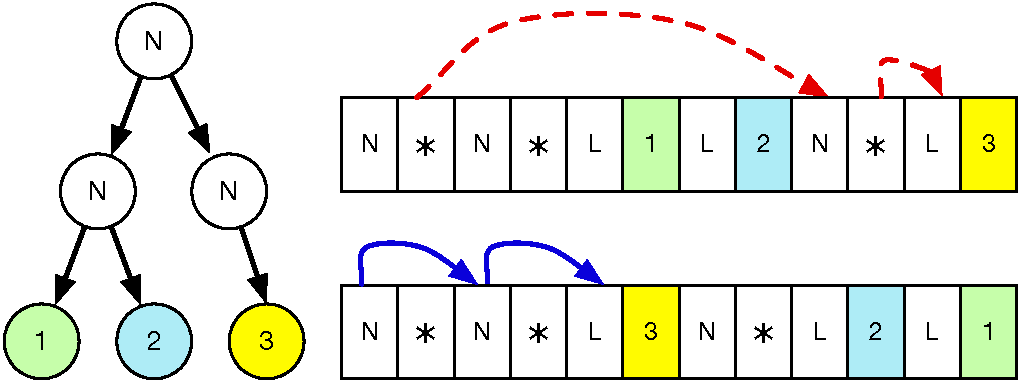
\includegraphics[width=0.6\linewidth]{figures/TreeShapedData.pdf}
	\caption{Rightmost: access patterns for, left-to-right (top) and right-to-left (bottom) serializations}
	\label{fig:treeShapedData}
\end{figure}

\subsection{Binary Tree Benchmarks}%
\label{subsec:trees}\label{subsec:eval:trees:rightmost}

We evaluate \system on a few binary tree benchmarks: adding one to all values in a tree,
exponentiation on integers stored in internal nodes, copying a tree and getting the right-most leaf value in the tree.
For the first three benchmarks, the tree representation we use is:
\begin{lstlisting}[]
  data Tree = Leaf | Node Int Tree Tree
\end{lstlisting}
For right-most, the tree representation we use is:
\begin{lstlisting}[]
  data Tree = Leaf Int | Node Tree Tree
\end{lstlisting}

\begin{table}
    \small
    \setlength{\tabcolsep}{4pt} %% default is 6pt
    \centering
	\caption{Run-time mean and 95\% confidence interval (ub, lb) for different
      layouts and traversal orders in the binary tree benchmarks (seconds).
              \misalignedPre{} -- post-order traversal on the pre-order layout of the tree.
              \misalignedPost{} -- pre-order traversal on the post-order layout of the tree.
              \alignedPre{} -- pre-order traversal on the pre-order layout of the tree.
              \alignedIn{} -- in-order traversal on an in-order layout of the tree.
              \alignedPost{} -- post-order traversal on the post-order layout of the tree.
              }
    \begin{tabular}{@{}lrrrrrrr@{}}
        \toprule
        \multirow{2}[2]{*}{\thead[l]{Benchmark\\name}}
        & \multicolumn{5}{c}{{\gibbon}}
        & \multicolumn{2}{c}{{\system}}\\
        \cmidrule(lr){2-6}\cmidrule(lr){7-8}
        & \multicolumn{1}{c}{\scriptsize{\misalignedPre}}
        & \multicolumn{1}{c}{\scriptsize{\misalignedPost}}
        & \multicolumn{1}{c}{\scriptsize{\alignedPre}}
        & \multicolumn{1}{c}{\scriptsize{\alignedIn}}
        & \multicolumn{1}{c}{\scriptsize{\alignedPost}}
        & \multicolumn{1}{c}{\scriptsize{\systemGreedy}}
        & \multicolumn{1}{c}{\scriptsize{\systemSolver}}\\
     \midrule
      \thead[l]{%
        \benchname{AddOneTree}
		\\\vspace{0cm}}
            & \thead{\textcolor{\myred}{{45.51}}\\ \scriptsize{(45.35, 45.66)}}
            &   \thead{memory\\error}
            &   \thead{{{1.29}}\\ \scriptsize{(1.29, 1.29)}}
    		&   \thead{{{1.30}}\\ \scriptsize{(1.30, 1.30)}}
    		&   \thead{{{1.29}}\\ \scriptsize{(1.29, 1.29)}}
    		&   \thead{{{1.29}}\\ \scriptsize{(1.29, 1.29)}}
            &   \thead{\textcolor{\myblue}{{1.28}}\\ \scriptsize{(1.28, 1.28)}}
            \\
      \thead[l]{%
        \benchname{ExpTree}
		\\\vspace{0cm}}
            & \thead{\textcolor{\myred}{{45.52}}\\ \scriptsize{(45.34, 45.70)}}
            &   \thead{memory\\error}
            &  \thead{{\fnumtwo{1.3119424788732397}}\\ \scriptsize{(\fnumtwo{1.3118021074983999}, \fnumtwo{1.3120828502480795})}}
    		&   \thead{{\fnumtwo{1.3128224647887325}}\\ \scriptsize{(\fnumtwo{1.312729018973989}, \fnumtwo{1.312915910603476})}}
    		&   \thead{{\fnumtwo{1.2938285633802817}}\\ \scriptsize{(\fnumtwo{1.2937382563056141}, \fnumtwo{1.2939188704549494})}}
    		&   \thead{{\fnumtwo{1.3117947323943662}}\\ \scriptsize{(\fnumtwo{1.311661357137603}, \fnumtwo{1.3119281076511293})}}
            &   \thead{\textcolor{\myblue}{\fnumtwo{1.292822605633803}}\\ \scriptsize{(\fnumtwo{1.2919551360395027}, \fnumtwo{1.2936900752281033})}}
            \\
      \thead[l]{%
        \benchname{CopyTree}
		\\\vspace{0cm}}
            & \thead{\textcolor{\myred}{{45.52}}\\ \scriptsize{(45.37, 45.67)}}
            &   \thead{memory\\error}
            &  \thead{{\fnumtwo{1.2870960563380283}}\\ \scriptsize{(\fnumtwo{1.286875053013491}, \fnumtwo{1.2873170596625656})}}
    		&   \thead{{\fnumtwo{1.2969579436619716}}\\ \scriptsize{(\fnumtwo{1.2967934277469406}, \fnumtwo{1.2971224595770026})}}
    		&   \thead{{\fnumtwo{1.2786742816901409}}\\ \scriptsize{(\fnumtwo{1.2785930976634212}, \fnumtwo{1.2787554657168605})}}
    		&   \thead{{\fnumtwo{1.2858431830985915}}\\ \scriptsize{(\fnumtwo{1.2857585274482104}, \fnumtwo{1.2859278387489725})}}
            &   \thead{\textcolor{\myblue}{\fnumtwo{1.2766249295774648}}\\ \scriptsize{(\fnumtwo{1.2765012665588478}, \fnumtwo{1.2767485925960818})}}
            \\
    \bottomrule
    \end{tabular}
    \label{table:Add-one-Tree}
    \label{table:Exponentiation-Tree}
	\label{table:Copy-Tree}
\end{table}


\begin{description}

\item[AddOneTree]
This benchmark takes a full binary tree and increments the values stored in the internal nodes of the tree.
We show the performance of an aligned preorder, inorder and postorder traversal in addition to a misaligned 
preorder and postorder traversal of the tree. Aligned traversals are ones where the data representation exactly
matches the traversal order, for instance, a preorder traversal on a preorder representation of the tree. 
A misaligned traversal order is where the access patterns of the traversal don't match the data layout of the tree.
For instance, a postorder traversal on a tree serialized in preorder. 
Table~\ref{table:Add-one-Tree} shows the performance numbers.
\systemSolver picks the aligned postorder traversal order which is best performing. It makes the recursive calls to the left and right children of the
tree first and increments the values stored in the internal nodes once the recursive calls return. The tree representation is also changed to a postorder
representation with the \lstinline|Int| placed after the left and right children of the tree. 
This is in part due to the structure of arrays effect, as the \lstinline|Int| are placed closer to each other.
\systemGreedy on the other hand picks the 
aligned preorder traversal because of its greedy strategy which prioritizes placing the \lstinline|Int| before the left and right subtree.
The tree depth is set to 27. At this input size, the \misalignedPost traversal failed due to memory errors, and
\misalignedPre runs $\sim$35$\times$ slower than aligned versions because of the skewed access patterns of the traversal.

\item[ExpTree]
This traversal does exponentiation on the values stored in the internal nodes of the tree. It is more computationally intensive than incrementing the value.
We raise the \lstinline|Int| to a power of 10 on a tree of depth 27. Table~\ref{table:Exponentiation-Tree} shows the performance of the different layout and traversal orders.
\systemSolver picks the \alignedPost representation which is the best performing, whereas \systemGreedy picks the \alignedPre representation. 

\item[CopyTree]
Copy-tree takes a full binary tree and makes a fresh copy of the tree in a new memory location.
We use a tree of depth 27 in our evaluation. Table~\ref{table:Copy-Tree} shows the performance of different layout and traversal orders. 
We see that \alignedPost traversal performs the best. Indeed, \systemSolver picks the \alignedPost representation, whereas, \systemGreedy chooses the 
\alignedPre representation.

\item[Rightmost]%
This traversal does recursion on the right child of the tree and returns the \lstinline|Int| value stored in the right-most leaf of the tree.
%
Figure~\ref{fig:treeShapedData} shows an example of a tree with two different serializations of the tree: left-to-right (top) and right-to-left (bottom).
The right-to-left serialization is more efficient because the constant-step movements (blue arrows) are usually more favorable than variable-step ones (red arrows) on modern hardware.
%
Both \systemSolver and \systemGreedy pick the right-to-left serialization, and
Table~\ref{table:Right-Most-Tree} shows that this choice performs better in the benchmark.
%
% As the input, we use the largest tree size (depth of 32) we can on the testing machine.
% The running time of the benchmark is significantly lower than the time it takes to build the tree.
% It is \textit{logarithmic} in the number of nodes in the tree.
\end{description}

%\rn{And why was it a linked list of strings instead of a markup tree or a single string?}
%\vs{I'm not sure why it was entered as a list but its a Pandoc Blovk type.}
\subsection{Blog Software Case Study}
\label{subsect:blog}

The Blog software case study serves as an example of a realistic benchmark, representing a sample of components 
from a \new{blog management web service}. The main data structure \new{is a linked list of blogs where each blog
contains fields} such as header, ID, author information, content, hashtags and date. The fields are a mix
of recursive and non-recursive datatypes. For instance, \lstinline{Content} is a recursive type 
\new{(the Pandoc \lstinline|Block| type)}, but \lstinline{Author} is a single string wrapped in a data
constructor.\footnote{At times, we have to wrap scalars in data constructors to make them packed fields.~\gibbon
does not always support mixing scalar and packed fields due to compiler bugs.}
%\csk{clarify reasoning packed/non-packed fields.}
One possible permutation of fields in the blog is:
%
\begin{lstlisting}[ ]
  data Blogs = Empty|HIADCTB Header Id Author Date Content HashTags Blogs
\end{lstlisting} 
%
%% This datatype is recursive and essentially represents a list of blogs present in the Blog service. 
%% A packed representation of this datatype packs all the fields as close to each other in memory as possible.
%% We perform a few traversals over this data type and show that the layout in which fields are instantiated matters.

We evaluate \system{}'s performance using three different traversals over a list of blogs.
%
Overall, the traversals accept a keyword and a list of blogs; in the
blogs, the traversals inspect either of the three fields: \lstinline{Content},
\lstinline{HashTags}, and the tail of the linked-list, \lstinline{Blogs}.
(Since \lstinline{Blogs}, \lstinline{Content}, and \lstinline{HashTags} are
recursive fields, changing their layout should represent greater differences in performance.)
%
The fields used by an individual traversal are referred as {\em active fields}
and the rest are referred as {\em passive fields}, and we specify these per-traversal below.

In Table~\ref{table:blog-traversals}, we report the performance of the six
possible layouts obtained by permuting the order of the three recursive fields,
and two additional layouts (Columns 1 and 2).
%
The column names indicate the order of fields used;
%
for example, the column \lstinline{hiadctb} reports numbers for the layout with fields ordered as:
\lstinline{Header}, \lstinline{Id}, \lstinline{Author}, \lstinline{Date}, \lstinline{Content}, \lstinline{HashTags}, and \lstinline{Blogs}.
%
All run times are gathered with \gibbon{}, and
%% \footnote{Since \system builds on \gibbon, this is equivalent to running \system with a flag that disables its field reordering optimization.} 
%
%% The column named \system{}
last two columns show the run times for code compiled using \system's greedy
and solver-based optimization, respectively.
%
%\system picks a layout tailored to each traversal, which we specify below.
%
%% We show the run-times of different traversals over a subset permutation of layouts for the Blog data structure when compiled with \gibbon . We compile the Blog data type with \system and show its performance for comparison.


\begin{table}[]
\small
\setlength{\tabcolsep}{1pt} %% default is 6pt
\centering
	\caption{Run-time mean and 95\% confidence interval (ub, lb) for different layouts in the blog software benchmarks (seconds).
		Several possible permutations of layout are shown.
		Layout names abbreviations: h -- Header, t -- HashTags, b -- Blogs, i -- TagID, c -- Content, a -- Author, d -- Date.}%
\label{table:blog-traversals}
\begin{tabular}{@{}p{7mm}rrrrrrrrrrr@{}}
\toprule
\multirow{2}[2]{*}{\thead[l]{\scriptsize Bench.\\\scriptsize name}}
 & \multicolumn{7}{c}{{\gibbon}}
 & \multicolumn{2}{c}{{\system}}\\
 \cmidrule(lr){2-8}\cmidrule(lr){9-10}
 %
 & \multicolumn{1}{c}{\small{{hiadctb}}}
 & \multicolumn{1}{c}{\small{{ctbhiad}}}
 & \multicolumn{1}{c}{\small{{tbchiad}}}
 & \multicolumn{1}{c}{\small{{tcbhiad}}}
 & \multicolumn{1}{c}{\small{{btchiad}}}
 & \multicolumn{1}{c}{\small{{bchiadt}}}
 & \multicolumn{1}{c}{\small{{cbiadht}}}
 & \multicolumn{1}{c}{\small{\systemGreedy}}
 & \multicolumn{1}{c}{\small{\systemSolver}}\\ 
\midrule
\benchname{FilterBlogs} \\
        &  \thead{\fnumtwo{0.2247852661971830}\\ \scriptsize{(\fnumtwo{0.22474188311863516}, \fnumtwo{0.22482864927573096})} }       
		&  \thead{\fnumtwo{0.2243197802816901}\\ \scriptsize{(\fnumtwo{0.22373525904937216}, \fnumtwo{0.22490430151400806})} }
		&  \thead{{\fnumtwo{0.08109379788732393}}\\ \scriptsize{(\fnumtwo{0.08082428580616613}, \fnumtwo{0.08136330996848173})} }
		&  \thead{\fnumtwo{0.26502487464788727}\\ \scriptsize{(\fnumtwo{0.26470682674275325}, \fnumtwo{0.2653429225530213})} }
		&  \thead{\fnumtwo{0.28165434366197184}\\ \scriptsize{(\fnumtwo{0.28142152424862715}, \fnumtwo{0.2818871630753165})} }
		&  \thead{\textcolor{\myred}{\fnumtwo{0.29489771690140854}}\\ \scriptsize{(\fnumtwo{0.29456292511661414}, \fnumtwo{0.29523250868620293})} }
		&  \thead{{\fnumtwo{0.2125426746478873}}\\ \scriptsize{(\fnumtwo{0.2122561149597799}, \fnumtwo{0.21282923433599468})} }
		&  \thead{{\fnumtwo{0.07244831014084505}}\\ \scriptsize{(\fnumtwo{0.07198399286596101}, \fnumtwo{0.07291262741572908})} }
		&  \thead{\textcolor{\myblue}{\fnumtwo{0.05624464183098592}}\\ \scriptsize{(\fnumtwo{0.05621462653189447}, \fnumtwo{0.056274657130077364})} }
		\\
        \\
\benchname{EmphContent}\\
&  \thead{\fnumtwo{0.6727033126760564}\\ \scriptsize{(\fnumtwo{0.6722382387120264}, \fnumtwo{0.6731683866400865})} }
&  \thead{\fnumtwo{0.6501001084507042}\\ \scriptsize{(\fnumtwo{0.6498550137449516}, \fnumtwo{0.6503452031564568})} }
&  \thead{\fnumtwo{1.5980927323943663}\\ \scriptsize{(\fnumtwo{1.5977151332795287}, \fnumtwo{1.598470331509204})} }
&  \thead{\fnumtwo{0.6631653633802816}\\ \scriptsize{(\fnumtwo{0.6629708671325513}, \fnumtwo{0.663359859628012})} }
&  \thead{\textcolor{\myred}{\fnumtwo{1.6327312253521127}}\\ \scriptsize{(\fnumtwo{1.6322556594551008}, \fnumtwo{1.6332067912491246})} }
&  \thead{\fnumtwo{1.6106063239436619}\\ \scriptsize{(\fnumtwo{1.6100967763696805}, \fnumtwo{1.6111158715176432})} }
&  \thead{\fnumtwo{0.4718713577464788}\\ \scriptsize{(\fnumtwo{0.4717313650476324}, \fnumtwo{0.4720113504453252})} }
&  \thead{\textcolor{\myblue}{\fnumtwo{0.4662895661971831}}\\ \scriptsize{(\fnumtwo{0.4661310844342112}, \fnumtwo{0.466448047960155})} }
&  \thead{\fnumtwo{0.6406900507042251}\\ \scriptsize{(\fnumtwo{0.640593687233358}, \fnumtwo{0.6407864141750923})} }
\\
\\
\benchname{TagSearch} \\
&  \thead{\fnumtwo{1.9893401126760561}\\ \scriptsize{(\fnumtwo{1.9890376935881537}, \fnumtwo{1.9896425317639586})} }
&  \thead{\fnumtwo{1.9794032253521132}\\ \scriptsize{(\fnumtwo{1.979185046541394}, \fnumtwo{1.9796214041628324})} }
&  \thead{\fnumtwo{3.2946498450704222}\\ \scriptsize{(\fnumtwo{3.2926928080206848}, \fnumtwo{3.2966068821201597})} }
&  \thead{\fnumtwo{1.6800026760563378}\\ \scriptsize{(\fnumtwo{1.679670088341037}, \fnumtwo{1.6803352637716387})} }
&  \thead{\textcolor{\myred}{\fnumtwo{3.3090972676056336}}\\ \scriptsize{(\fnumtwo{3.308674578901536}, \fnumtwo{3.3095199563097313})} }
&  \thead{\fnumtwo{3.3028858732394366}\\ \scriptsize{(\fnumtwo{3.302365980422784}, \fnumtwo{3.3034057660560894})} }
&  \thead{\fnumtwo{1.8170195492957746}\\ \scriptsize{(\fnumtwo{1.8164916768029753}, \fnumtwo{1.8175474217885739})} }
&  \thead{\fnumtwo{1.7559784788732393}\\ \scriptsize{(\fnumtwo{1.7555039213525125}, \fnumtwo{1.756453036393966})} }
&  \thead{\textcolor{\myblue}{\fnumtwo{1.736654943661972}}\\ \scriptsize{(\fnumtwo{1.736380487003441}, \fnumtwo{1.7369294003205031})} }
\\
\bottomrule
\end{tabular}
\end{table}


%\subsubsection{{\bf FilterBlogs}}

\begin{description}

\item[FilterBlogs]
filters the list of blogs and only retains those which contain the given
keyword in the \lstinline{HashTags} field. %\csk{should describe what HashTags field is above.}
%% This traversal searches for a word queried by the user and returns all the blogs from the list of blogs in the service that have that keyword in the list of HashTags maintained by a blog. This traversal is essentially a \textit{map} over the blogs with the function (\textit{f}) that is passed to map having the type signature of \textit{(String -> Blogs -> Maybe Blogs)}. \textit{f} takes the queried keyword, the old Blog and returns the old Blog if this keyword is present in the HashTags list.
%
%%  Therefore, in table~\ref{table:blog-traversals} we show the performance of the permutations of the layouts where these fields are shuffled around when compiled with \gibbon. The last column shows the performance of the layout chosen by \system.
%
%% This traversal makes use of only the \lstinline{HashTags} and \lstinline{Blogs} fields. We refer to these fields as ``active fields''. The rest of the fields are unused and we call these ``passive fields''.
%
\new{The {\em active fields} for this traveral are \lstinline{HashTags} and \lstinline{Blogs}.}
%
Theoretically, the performance of this traversal is optimized when the \lstinline{HashTags} field is serialized before \lstinline{Blogs} on account of the first access to \lstinline{HashTags} in the traversal.
%
%% As expected the layout \textbf{\textit{tbchiad}} gives the best performance when compiled with \gibbon.
This is confirmed in practice with the layout \textbf{\textit{tbchiad}} being the fastest.
%
% The access to \lstinline{HashTags} comes first since its serialized first in memory and once HashTags is fully traversed, the traversal can access blogs in an optimal manner without unnecessary movement in the packed buffer.
%
\system chooses the layout with \lstinline{HashTags} serialized first and followed by \lstinline{Blogs};
\new{
  the order of other fields remains unchanged compared to the source program,
  but this has no effect on performance since they are {\em passive fields}.
}
%% does not matter since they are passive fields and \new{their new order depends on their initial order specified in the program.}
%% it depends on the order of these fields in the initial layout given to \system to optimize.
Table~\ref{table:blog-traversals} also shows that layout chosen by \system performs similar to the layout \textbf{\textit{tbchiad}}.
Both \systemSolver and \systemGreedy pick the layout \textbf{\textit{tbhiadc}} when compiled from the initial layout \textbf{\textit{hiadctb}}.

%% \subsubsection{Traversal2: Emphasize a word queried in the content:}
%\subsubsection{{\bf EmphContent}}

\item[EmphContent]
%This traversal takes a keyword and a list of blogs as input. It then
searches the content of each blog for the keyword and emphasizes all its occurrences there (if any).
%
%% This traversal does this recursively for all the blogs in the program. This traversal is a map where the supplied function(\textit{f}) has the type signature of \textit{(String -> Blogs -> Blogs)}. It takes a keyword to be emphasized in the Content fields, the old Blogs and returns the Blogs with either the new content if the keyword is present or leave the content unchanged if it is not present in the content. 
%
The active fields in this traversal are \lstinline{Content} and \lstinline{Blogs}.
Based on the access pattern (\lstinline{Content} accessed before \lstinline{Blogs}),
the layout with the best performance should place \lstinline{Content} first followed by \lstinline{Blogs}.
In practice, the layout with the best performance is \textbf{\textit{cbiadht}}.
In contrast, \systemSolver prioritizes the placement of \lstinline{Blogs} before \lstinline{Content}, but
it also changes the traversal to recurse on the blogs first and then emphasize content.
%% placing it Content first followed by Blogs.
The passive fields are placed afterwards.
The layout chosen by \systemSolver is \textbf{\textit{bchiadt}}, whereas the layout chosen by \systemGreedy is \textbf{\textit{cbhiadt}} when compiled from the initial layout \textbf{\textit{hiadctb}}.
The performance of \systemGreedy and
\systemSolver differ because datatypes other than \lstinline{Blogs} differ in their layout choices.

%% \subsubsection{Traversal3: Search a keyword in HashTags and emphasize it in content:}
% \subsubsection{{\bf TagSearch}}

\item[TagSearch]
% This traversal takes a keyword and a list of blogs as input and
looks for the presence of the keyword in the \lstinline{HashTags} field, and
if the keyword is present, the traversal emphasizes the keyword in the \lstinline{Content}.
%
%% and depending on if its present or not emphasizes or leaves it unchanged in the Content field. This traversal does this recursively for all the blogs in the program. 
%
%% This traversal is a map over the blogs with the supplied function(\textit{f}) having the type signature of \textit{(String -> Blogs -> Blogs)}. It takes a keyword, searches it 
%% in the HashTags and if it is present in the HashTags, emphasizes it in the Content field. The active fields in this traversal are HashTags, Content and Blogs. 
%
The layout with the best performance is
\textbf{\textit{tcbhiad}} because of the
access pattern, which inspects \lstinline{HashTags} followed by \lstinline{Content} followed by \lstinline{Blogs}.
\systemSolver chooses the layout \textbf{\textit{tbchiad}}---which places \lstinline|HashTags| followed by \lstinline|Blogs|
followed by \lstinline|Content|---and changes the traversal to recurse on \lstinline|Blogs| first and later emphasize
\lstinline|Content| in the \lstinline|then| branch.
On the other hand, \systemGreedy chooses \textbf{\textit{tcbhiad}}
when compiled from the initial layout \textbf{\textit{hiadctb}}.
%\system's performance is better and shows the effectiveness of the optimization.

%The layout \system chooses also places these fields in the same order. The performance as shown in Table~\ref{table:blog-traversals} and is similar to \textbf{\textit{tcbhiad}}. 

\end{description}

\subsubsection{\bf Globally optimizing multiple functions}

%\vs{TODO: add layout of solver and greedy version.}
We use \system to globally optimize the three blog traversals we discussed above such that we pick one layout for all traversals that minimizes the overall runtime. Table~\ref{table:global-blog-traversals} shows the runtime for a layout we compiled using \gibbon (\textit{\textbf{hiadctb}}), \systemSolver(\textit{\textbf{tbchiad}}) 
and \systemGreedy(\textit{\textbf{tbchiad}}). We see that \systemGreedy and \systemSolver do a good job in reducing the traversal time globally. 
All the three traversals are run in a pipelined fashion sequentially. Although, \systemSolver does worse with \textit{TagSearch} when run in a pipelined manner, 
it is actually better performing with \systemSolver when run alone as seen in table~\ref{table:blog-traversals}. 
Note that \systemSolver changes more that one data constructor based on the \textit{inlineable} attribute that \systemGreedy does not.
For instance, \systemSolver uses a packed \lstinline|Inline| list in the \lstinline|Content| with the tail serialized before \lstinline|Inline|.
Whereas, \systemGreedy uses a conventional packed list. In a pipelined execution of the traversals, although this helps reduce the runtime in the case 
of the content search traversal, it inadvertently increases the runtime in case of the tag search traversal due to a cache effect
that can benefit from runtime information.

\begin{table}
	\centering
	\caption{Run-time mean and 95\% confidence interval (ub, lb) for the blog
	  software benchmarks when \system optimizes the data layout globally (seconds).
           The input parameters are different from the single-function
		   optimization case.}%
\label{table:global-blog-traversals}
\begin{tabular}{@{}lrrr@{}}
	\toprule
    \multirow{2}[2]{*}{\thead[l]{Benchmark\\name}}
	& \multicolumn{1}{c}{{\gibbon}}
	& \multicolumn{2}{c}{{\system}}\\
    \cmidrule(lr){2-2}\cmidrule(lr){3-4}

	& \multicolumn{1}{c}{{hiadctb}}
	& \multicolumn{1}{c}{\small{\systemGreedy}}
	& \multicolumn{1}{c}{\small{\systemSolver}}\\
	\midrule
      \thead[l]{%
		\benchname{FilterBlogs}
		\\\vspace{0cm}}
			&  \thead{\textcolor{\myred}{\fnumtwo{2.230235366197183}}\\ \scriptsize{(\fnumtwo{2.2296601843214643}, \fnumtwo{2.230810548072902})}}
			& \thead{\fnumtwo{0.11155572676056338}\\ \scriptsize{(\fnumtwo{0.11129754268785376}, \fnumtwo{0.11181391083327301})}}
			& \thead{\textcolor{\myblue}{\fnumtwo{0.09500013323943661}}\\ \scriptsize{(\fnumtwo{0.0949635646349502}, \fnumtwo{0.09503670184392302})}}
			 \\
      \thead[l]{%
		\benchname{EmphContent}
		\\\vspace{0cm}}
		   &  \thead{\fnumtwo{1.5747499154929574}\\ \scriptsize{(\fnumtwo{1.5742668530634656}, \fnumtwo{1.5752329779224492})} }
		   & \thead{\textcolor{\myred}{\fnumtwo{1.3836891549295773}}\\ \scriptsize{(\fnumtwo{1.3835601882499424}, \fnumtwo{1.3838181216092122})} }
		   &  \thead{\textcolor{\myblue}{\fnumtwo{1.3222079577464787}}\\ \scriptsize{(\fnumtwo{1.3220798547722914}, \fnumtwo{1.322336060720666})} }
		   \\
      \thead[l]{%
		\benchname{TagSearch}
		\\\vspace{0cm}}
		   &  \thead{{\fnumtwo{2.196739676056339}}\\ \scriptsize{(\fnumtwo{2.196016148977572}, \fnumtwo{2.197463203135106})}}
		   &   \thead{\textcolor{\myblue}{\fnumtwo{1.830104352112676}}\\ \scriptsize{(\fnumtwo{1.828666212218745}, \fnumtwo{1.8315424920066072})}}
		   &   \thead{\textcolor{\myred}{\fnumtwo{2.3503619154929574}}\\ \scriptsize{(\fnumtwo{2.350152096698425}, \fnumtwo{2.35057173428749})}}
		   \\
   \bottomrule
   \end{tabular}
\end{table}


% \vs{The examples we have with the new cost model, this seems like a redundant section, maybe we remove this given 25 page limit for camera ready.}
% \subsubsection{{\bf tagSearch: varying likelihood of paths taken}}
% %
% % Traversal 3's
% TagSearch's source code is similar to our running example~\ref{fig:blog-travesal} where we
% %
% take different code paths
% % are traversing different paths
% based on if a keyword is present in the tags of the blog post or not. Thus, depending on which branch is more likely, different layouts of the Blog value can have different runtime performance. 

% This information cannot be inferred statically since the contents of the Blog is known only at runtime. This means that \system may not be able to generate an optimal layout on its own since it does not have the information about which branch is more likely via statically analyzing the structure of the program.
% %
% (As mentioned in \secref{sec:design}, we assume uniform likelihoods for branches if no information is provided.)

%\begin{table}[]
%\setlength{\tabcolsep}{0.1pt} %% default is 6pt
%\centering
%\ra{1}
%\begin{tabular}{@{}p{0.5in}rcrcr@{}}\toprule
%& \multicolumn{1}{c}{\textit{$Layout_{\tiny{\system(without\:\:pragma)}} $ }} & 
% & \multicolumn{1}{c}{$Layout_{\tiny{\system(with\:\:pragma)}}$ }\\ \midrule
%$Mdn$ & 0  &&   0 \\
%\bottomrule
%\end{tabular}
%\caption{Biasing the ``Then'' Branch for traversal 3: runtime in seconds for a subset permutation of different layouts when compiled with \gibbon .
%$Layout_{\system(without\:\:pragma)}$  shows the run-time for the layout chosen by \system without user supplied pragmas and $Layout_{\tiny{\system(with\:\:pragma)}}$ shows the run-time when the user supplies pragmas to branches. Legend: h - Header, t - HashTags, b - Blogs, i - TagID, c - Content, a - Author, d - Date}
%\end{table}


% \begin{table}[]
% \setlength{\tabcolsep}{0.1pt} %% default is 6pt
% \centering
% \ra{1}
% \begin{tabular}{@{}p{0.5in}rcrcr@{}}\toprule
% & \multicolumn{1}{c}{\textit{{\small{\systemSolver(without\:\:pragma)}} }} & 
%  & \multicolumn{1}{c}{{\textit{\small{\systemSolver(with\:\:pragma)}}} }\\ \midrule
% $Tag Search$ \\
% $Then$ & 1.707  &&  1.707 \\

% $Tag Search$ \\
% $Else$ & 0.0292  &&  0.0292 \\
% \bottomrule
% \end{tabular}
% \caption{Performance of traversal 3 (Tag Search) when the input is biased for either the ``Then'' or ``Else'' branch through the traversal. 
% {\small{\system(without\:\:pragma)}} shows the run-time for the layout chosen by \system without user supplied pragmas and {\small{\system(with\:\:pragma)}} shows the run-time when the user supplies likelihood values through pragmas in branches. The layout chosen in both the cases (with and without pragma is the same). Legend: h - Header, t - HashTags, b - Blogs, i - TagID, c - Content, a - Author, d - Date}
% \label{table:biasBranch}
% \end{table}


% \begin{table}[]
% \setlength{\tabcolsep}{0.1pt} %% default is 6pt
% \centering
% \ra{1}
% \begin{tabular}{@{}p{0.5in}rcrcr@{}}\toprule
% & \multicolumn{1}{c}{\textit{{\small{\system(without\:\:pragma)}} }} & 
%  & \multicolumn{1}{c}{{\textit{\small{\system(with\:\:pragma)}}} }\\ \midrule

% \bottomrule
% \end{tabular}
% \caption{Biasing the ``Else'' Branch for traversal 3 (TagSearch): Here we show the difference in performance when be bias the else branch of the traversal.
% {\small{\system(without\:\:pragma)}} shows the run-time for the layout chosen by \system without user supplied pragmas and {\small{\system(with\:\:pragma)}} shows the run-time when the user supplies likelihood values through pragmas in branches. Legend: h - Header, t - HashTags, b - Blogs, i - TagID, c - Content, a - Author, d - Date}
% \label{table:biasBranch}
% \end{table}




%\begin{table}[t]
%\centering
%\ra{1.3}
%\begin{tabular}{@{}rrrcrr@{}}\toprule
%& \multicolumn{2}{c}{Bias then branch} & & \multicolumn{2}{c}{Bias else branch} \\ 
%\cmidrule{2-3} \cmidrule{5-6}
%& \gibbon(s) & \system(s) && \gibbon & \system  \\ \midrule
%HIADCTB\\
%$M$     &    &     &&    &      \\
%$Mdn$ &    &      &&   &     \\
%CTBHIAD\\
%$M$     &    &      &&   &    \\
%$Mdn$ &   &      &&    &    \\
%\bottomrule
%\end{tabular}
%\caption{Runtime in seconds for case study where we vary the likelihood of branches in Traversal3. Legend: H - Header, T - HashTags, B - Blogs, I - TagID, C - Content, A - Author, D - Date}
%\vspace{-3em}
%\end{table}


%% However if the programmer has knowledge of which branch is more likely, we can use this knowledge to our advantage when ordering the fields of the data constructor. To this end, we could allow the programmer to specify which branch is more likely through \textit{annotation pragmas}\footnotemark{} in the source code. The programmer may specify the likelihood of particular branches while writing the traversal. If provided, \system could parse these and use them while generating the optimal layout of fields in the data constructor. 
%% \footnotetext{Currently \system does not provide the presence of such pragmas. Pragmas for the user to provide likelihoods are under development. The user provided likelihoods are currently hardcoded in the compiler in order to get the results}
% \rn{I don't like the speculative likelihood annotation thing... we would more likely just use profile data.}

% As a case study, we show the performance of the Blog data type for an input which biases both the ``Then'' and ``Else'' branch of the traversal separately. Without information on which branch is likely, \system produces a layout which has sub-optimal performance in the ``Else'' branch. The performance of this layout is shown in Table~\ref{table:biasBranch} in the {\small{\system(without\:\:pragma)}} column. This layout places HashTags first, followed by Content, Blogs and then the passive fields. Since the traversal goes to the ``Else'' branch, it has to jump over the Content fields serialized in between HashTags and Blogs resulting in poor performance. 

% When \system is given the information about which branch is likely, it generates a different layout where it places the HashTags field first, followed by Blogs, Content and finally the passive fields. This gives better performance as shown in the column {\small{\system(with\:\:pragma)}}  of table~\ref{table:biasBranch}.
% % 
% Since branch frequency from profiling data is a reasonable assumption, 
% % \system can be engineered easily to reason about the likelihoods if passed, it
% \system{} can generate more optimal layouts when compared to \gibbon. We also show the performance of the optimal layout generated by \system for the ``Then'' branch in \Figref{table:biasBranch}.

%\subsubsection*{When then branch is more likely in traversal~\ref{fig:blog-traversal}:}

%Here we provide a higher weight to the then branch in the source code which prioritizes the layout for the then branch. 


%\subsubsection*{When else branch is more likely in traversal~\ref{fig:blog-traversal}:}

%Here we provide a higher weight to the else branch in the source code which prioritizes the layout for the else branch.

%\subsubsection{Delete a keyword in HashTags: }
%
%This traversal takes a keyword to be deleted from the hash-tags of a Blog and a list of blogs as input. It traverses the hash-tags which is a linked-list of keywords and deletes the queried keyword in the hash-tags. 
%It does this recursively for all the blogs in the program. 

\begin{figure}[t]
\begin{minipage}[h]{.53\linewidth}
		\benchname{FilterBlogs}\\
		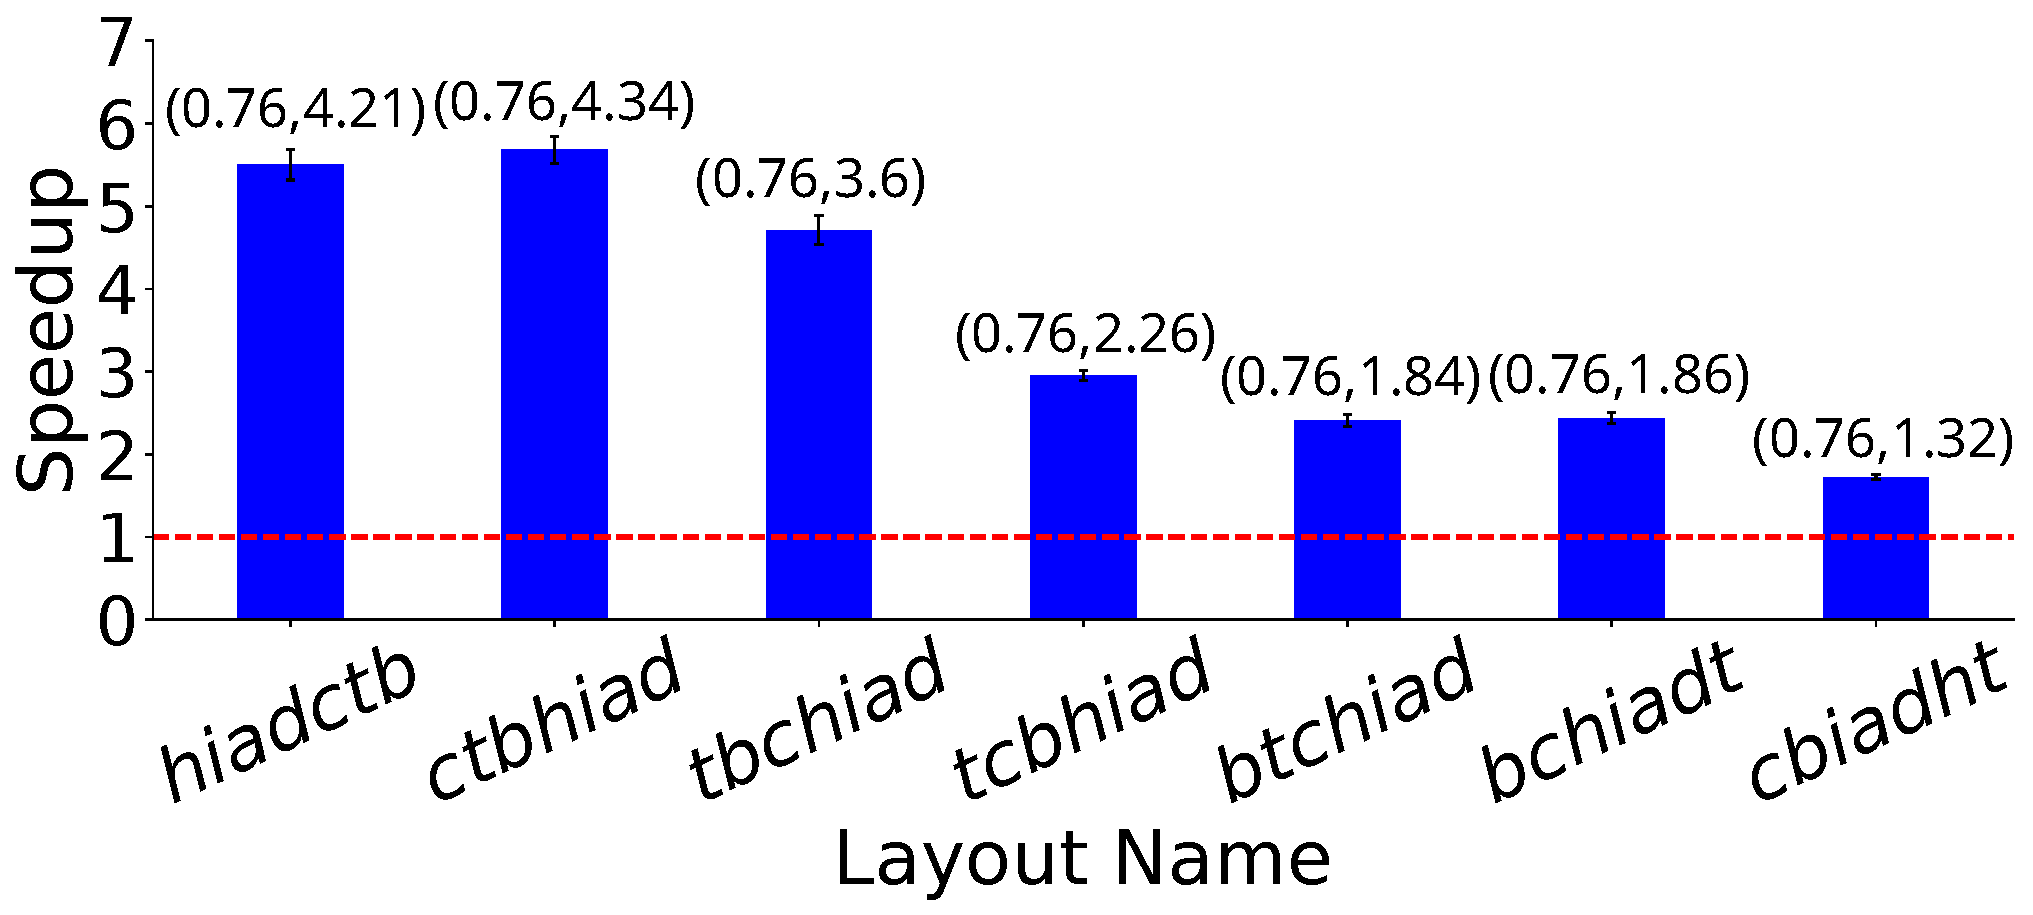
\includegraphics[width=\textwidth]{plots/SpeedupMarmosetSmlFilterBlogs}

		\benchname{EmphContent}\\
		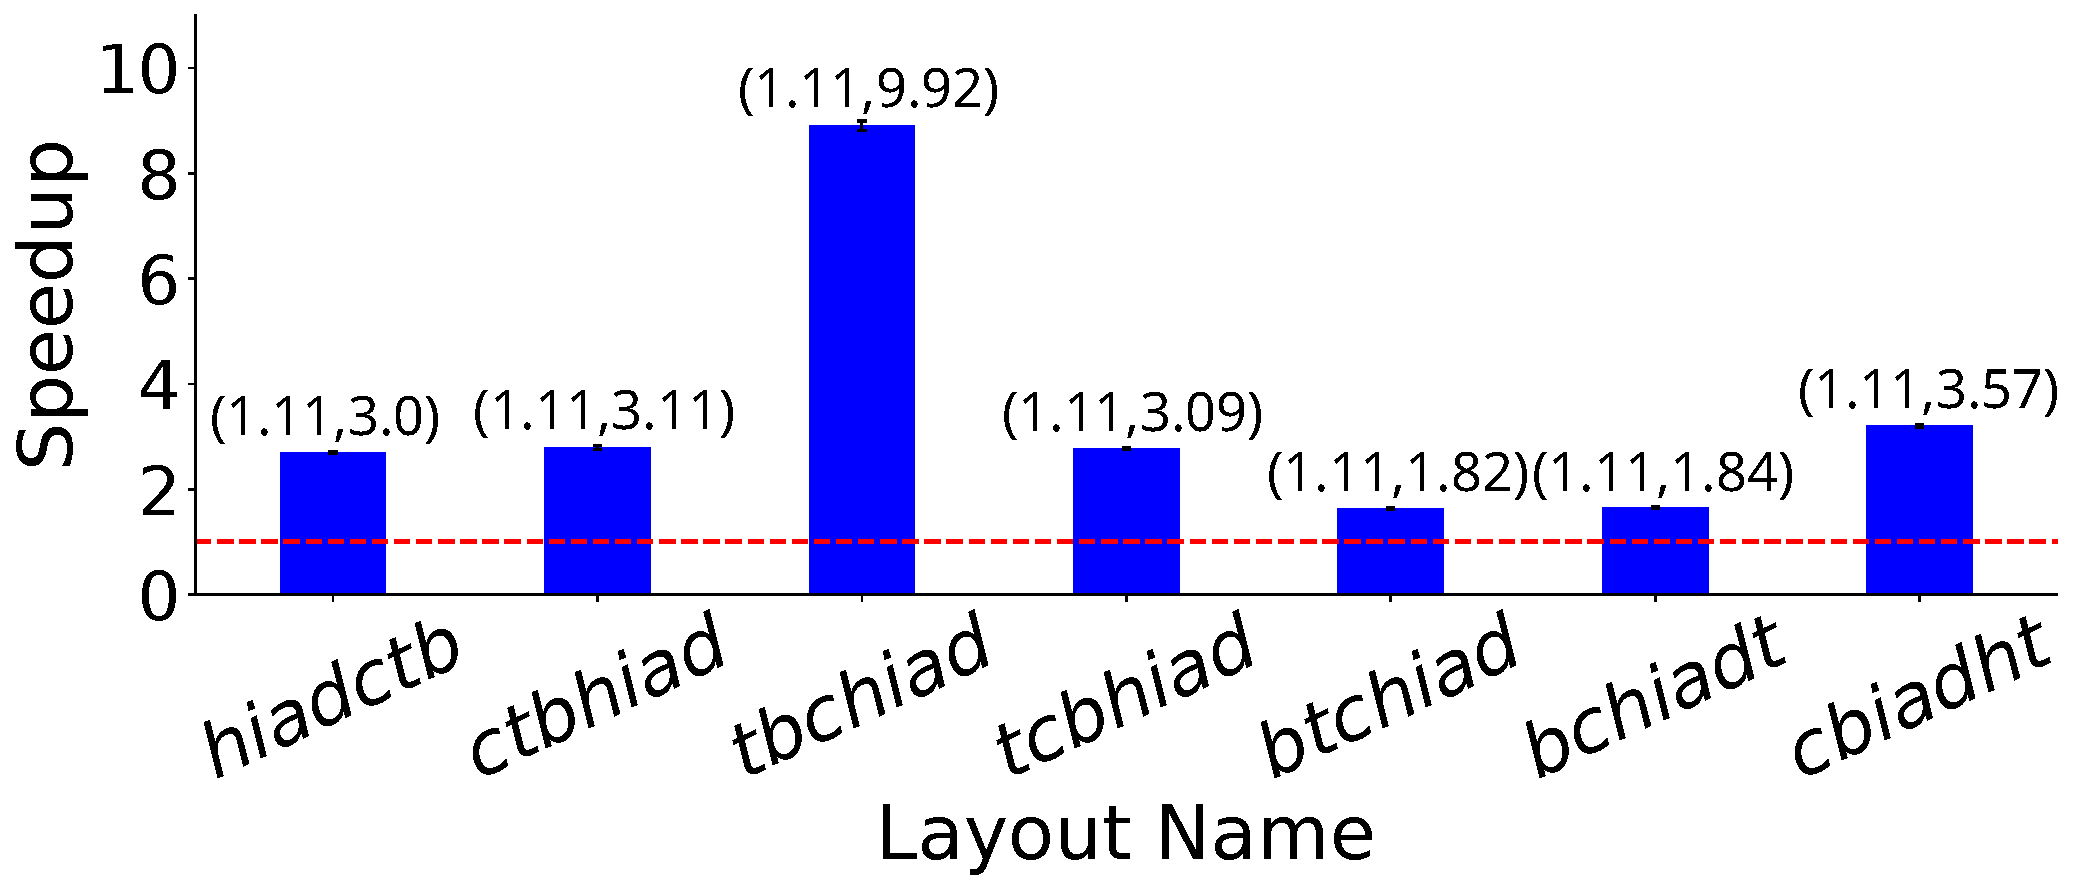
\includegraphics[width=\textwidth]{plots/SpeedupMarmosetSmlContentSearch}

		\benchname{TagSearch}\\
		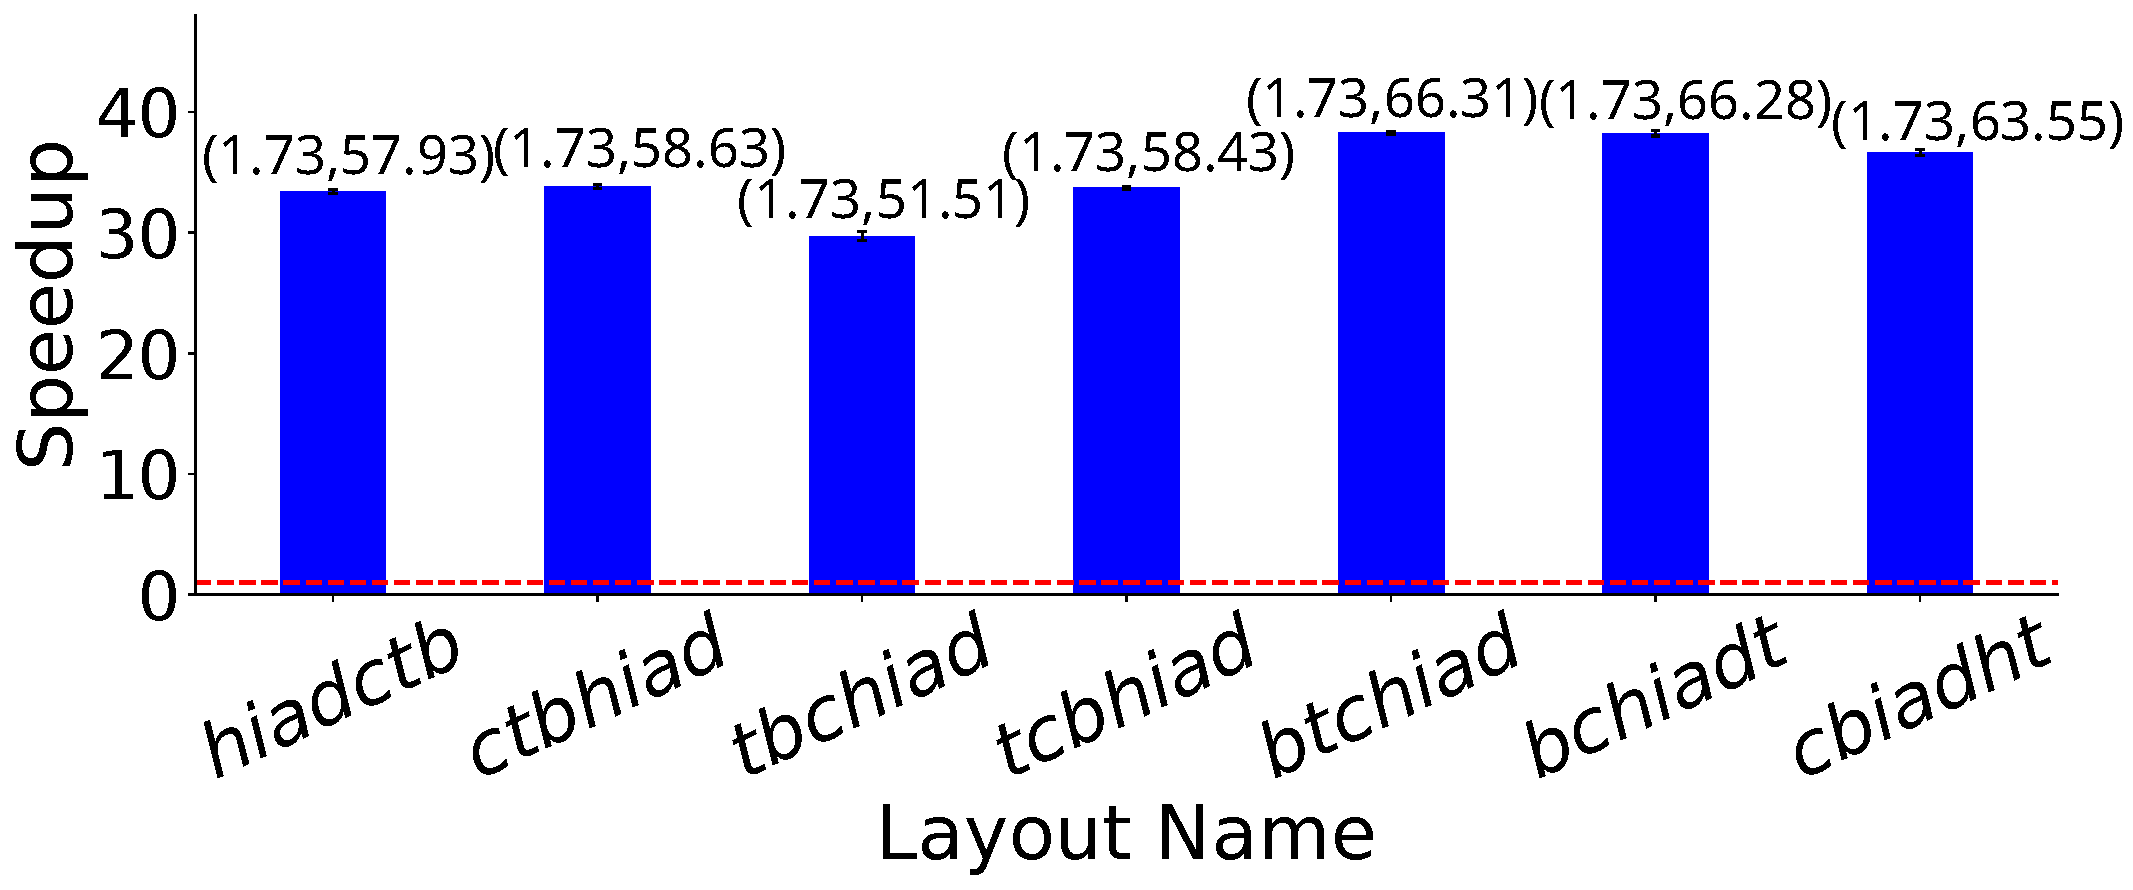
\includegraphics[width=\textwidth]{plots/SpeedupMarmosetSmlTagSearch}

	   \caption{Performance comparison of \systemSolver with \mlton.
	   The pair of numbers on top of each bar shows the median runtime in seconds of \systemSolver followed by the corresponding layout when compiled with \mlton.}
	   \label{fig:speedupghc}
\end{minipage}
\hfill
\begin{minipage}[h]{.44\linewidth}
		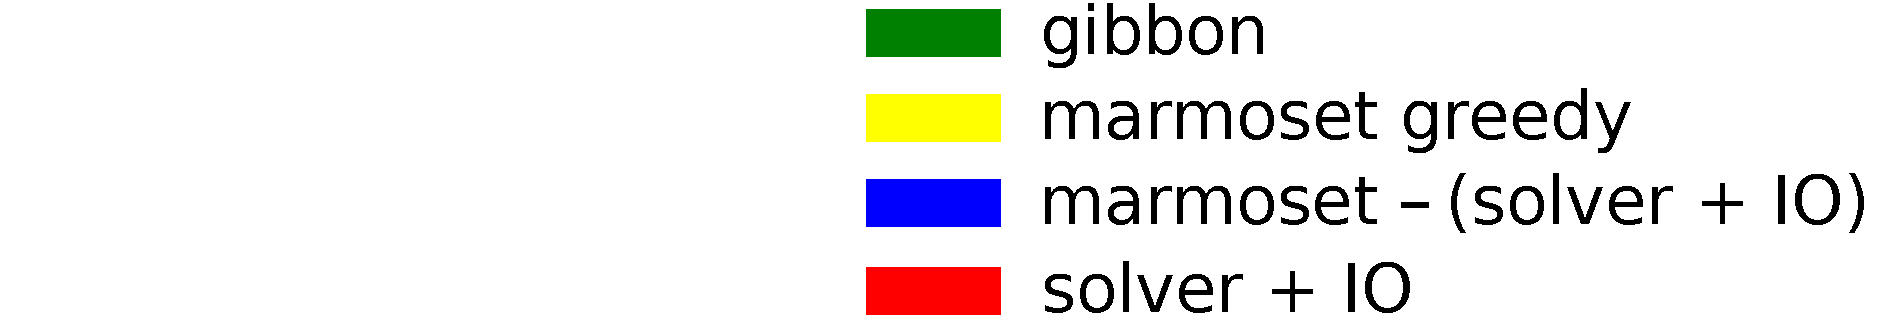
\includegraphics[width=.9\textwidth]{plots/CompileTimes-legend}

		\benchname{FilterBlogs}\\
		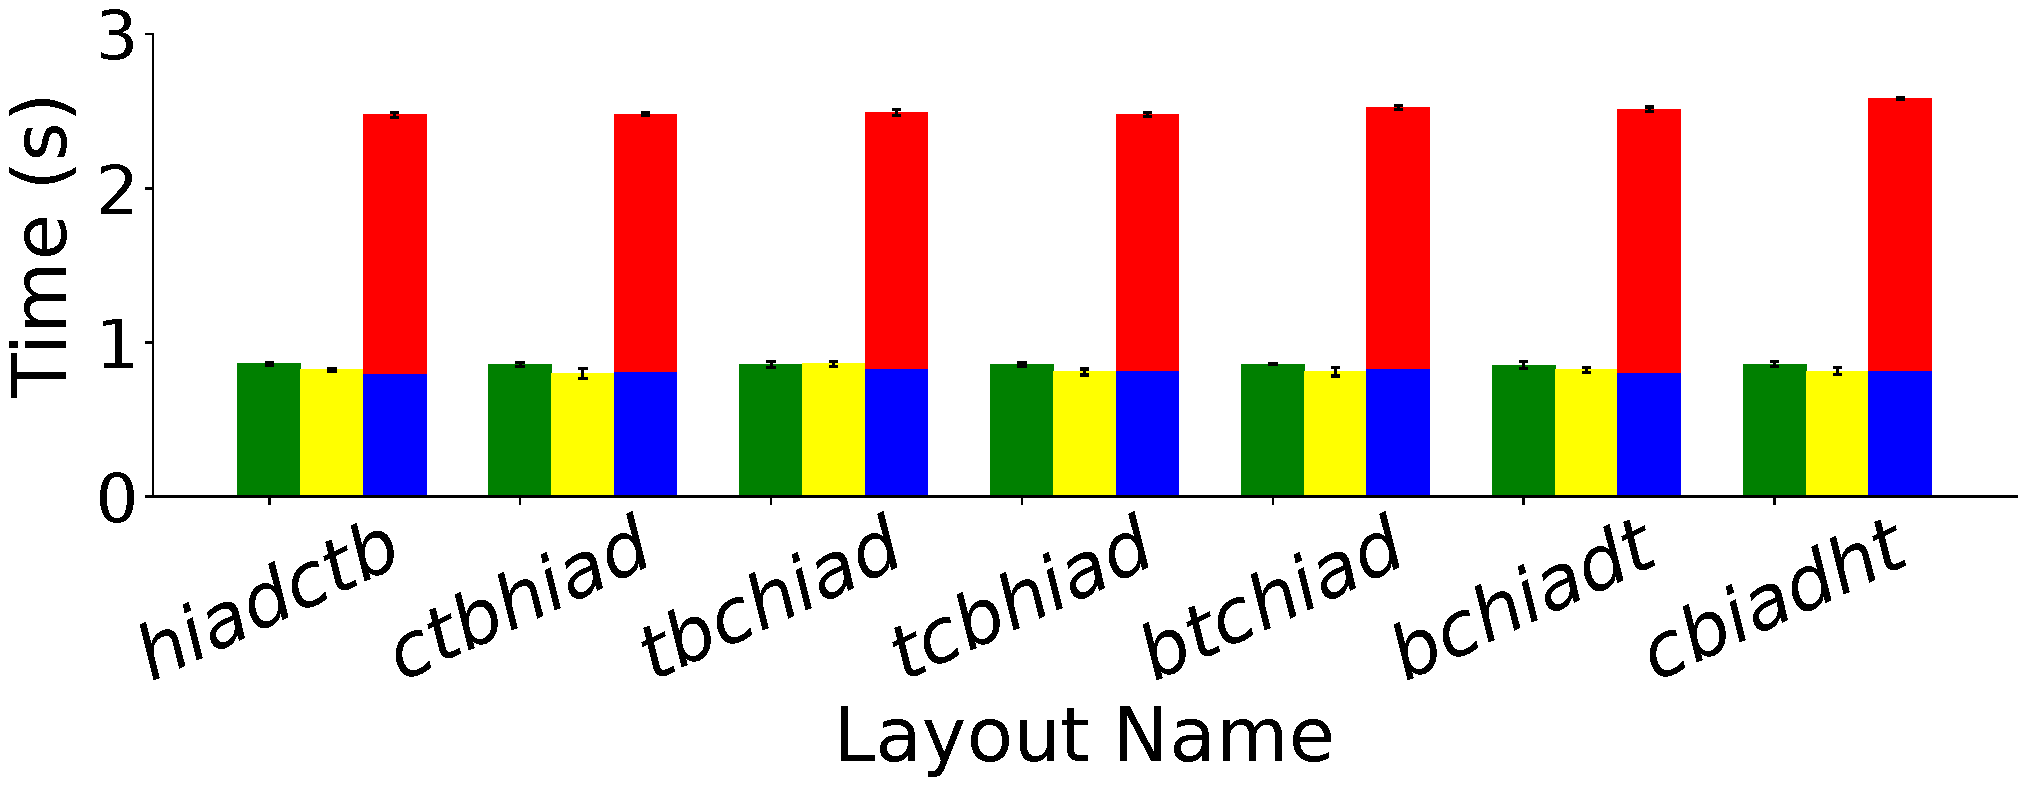
\includegraphics[width=\textwidth]{plots/FilterBlogCompileTimes-nolegend}

		\benchname{EmphContent}\\
		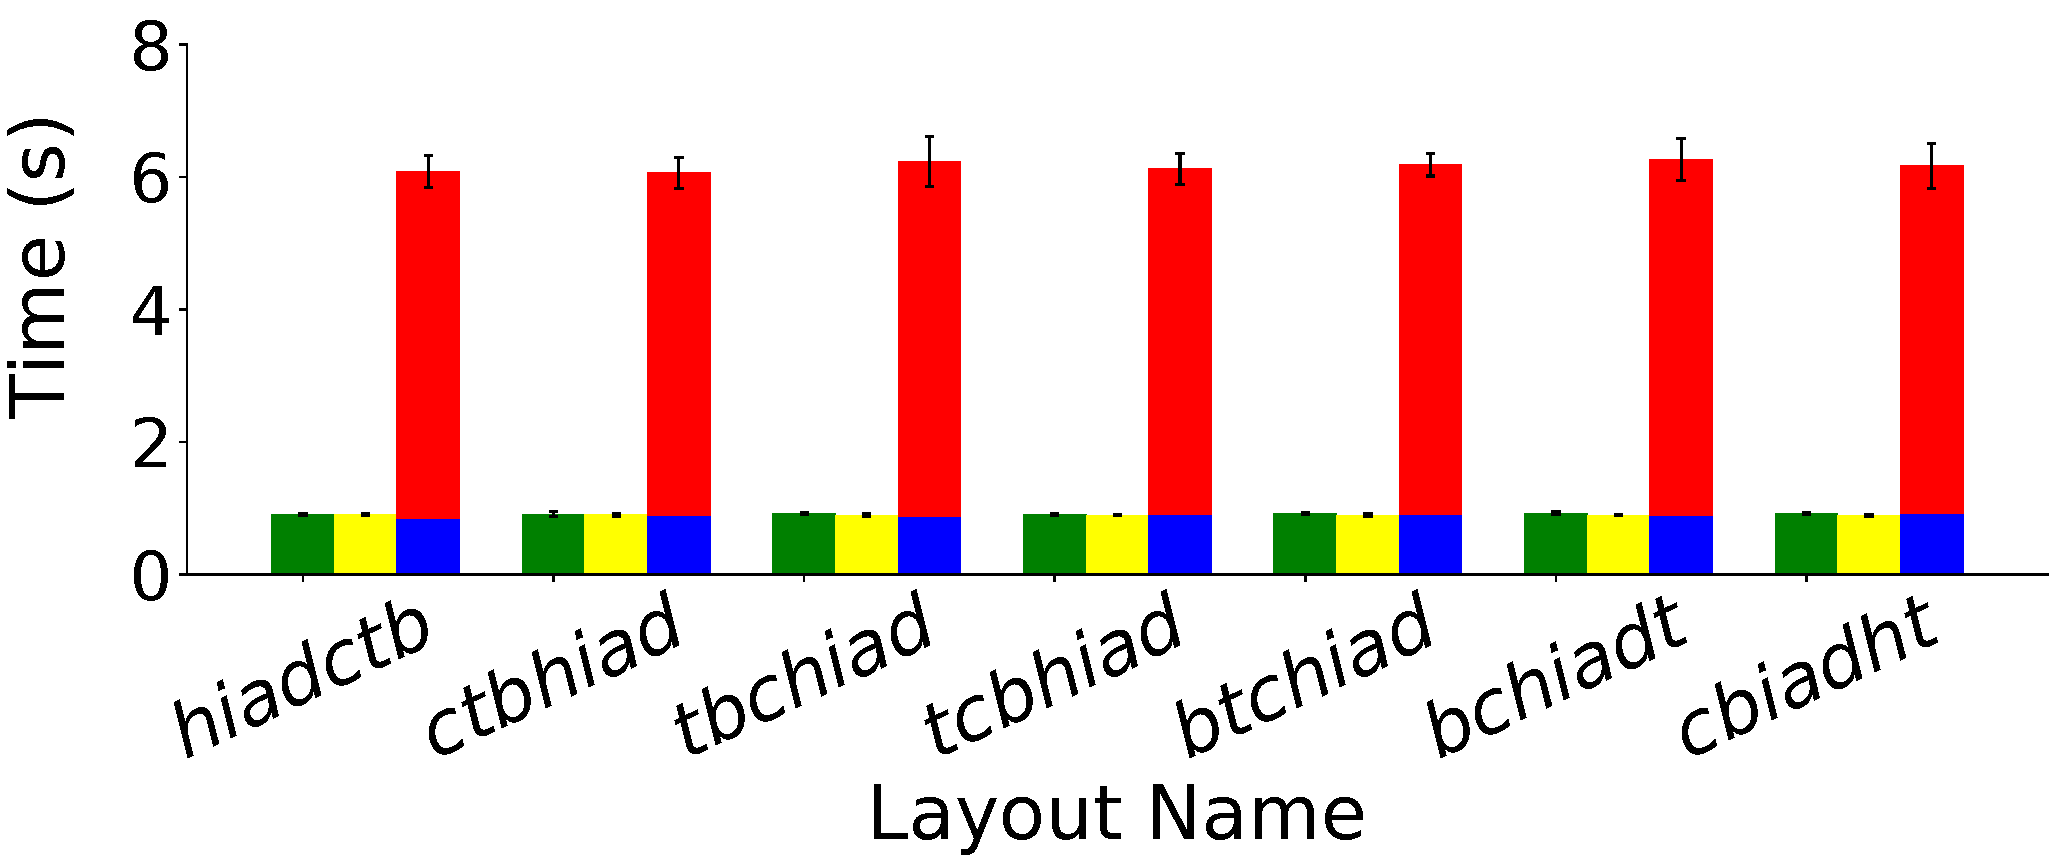
\includegraphics[width=\textwidth]{plots/ContentSearchCompileTimes-nolegend}

		\benchname{TagSearch}\\
		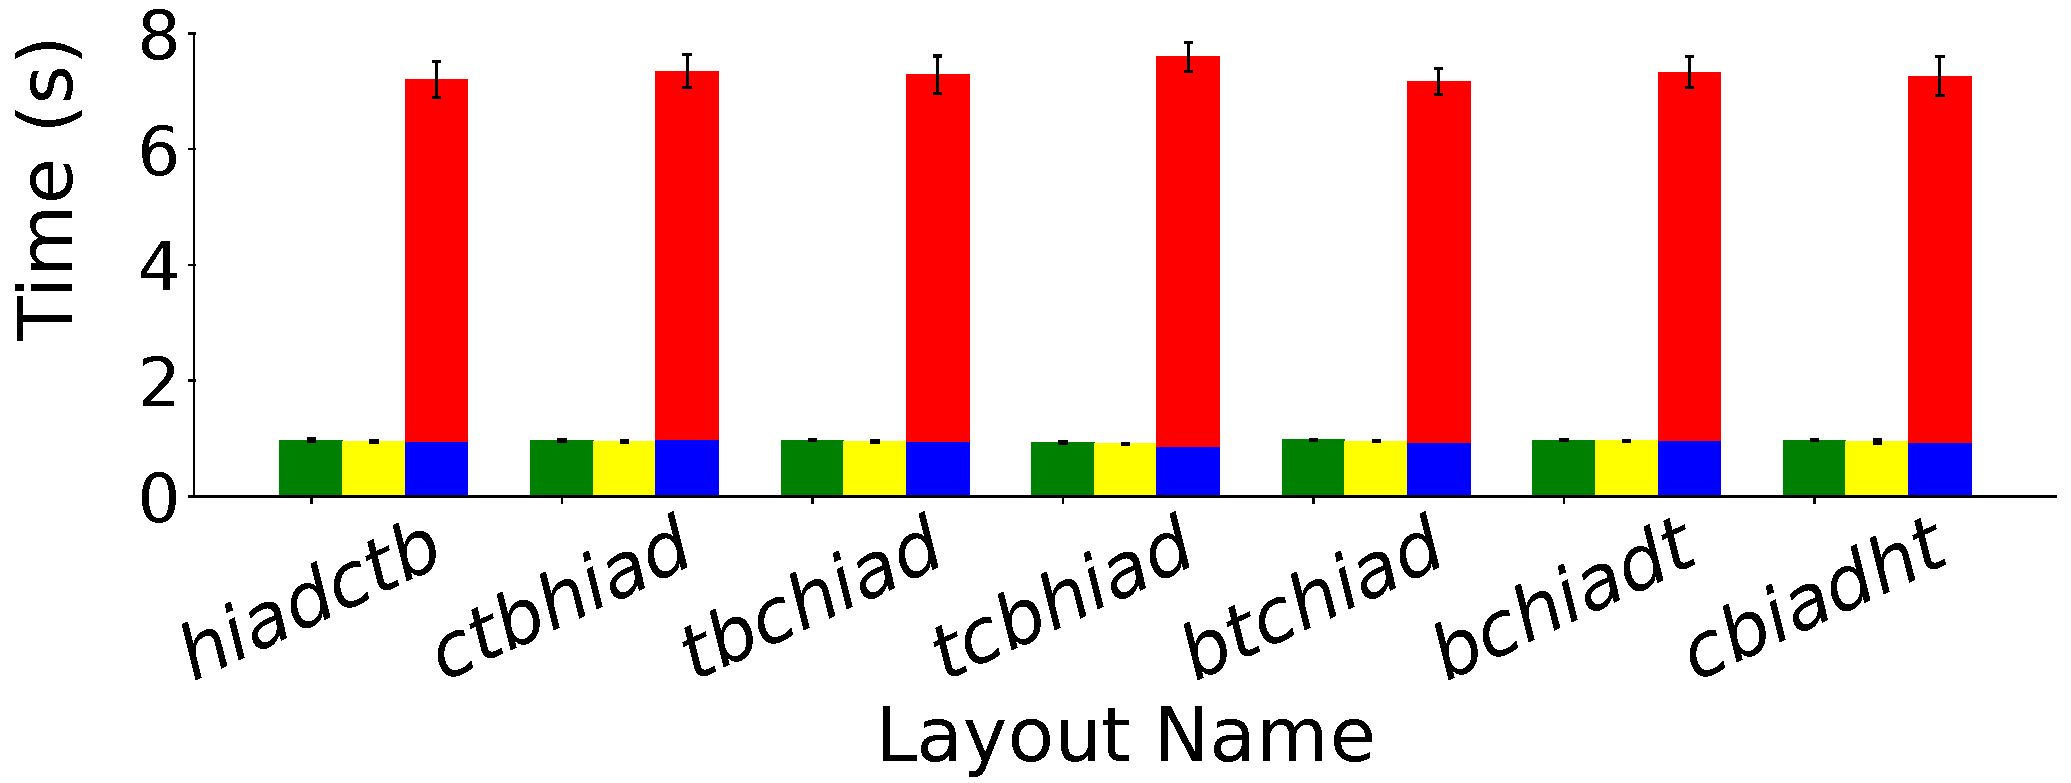
\includegraphics[width=\textwidth]{plots/TagSearchCompileTimes-nolegend}

	   \caption{
	             Average compile times (99 runs) in seconds for different layouts and traversal combinations
	   			 when compiled with \gibbon and when optimized by \systemGreedy and \systemSolver.
				 % The bar in \textit{Blue} is the time for \systemSolver after subtracting the
				 % time for solver IO and the bar in \textit{Red} is the time taken to do the IO call to the
				 % DOCPLEX solver. The total compile time for \systemSolver includes the time for doing the CFG
				 % analysis, generating the access graph, the solver time, reordering the datatype and repairing
				 % the code, The majority of which is added by the solver IO.
				 }
	   \label{table:compiletimes}
\end{minipage}
\end{figure}


\subsubsection{{\bf Comparison of \system against \mlton}}
\label{subsec:mlton}

We compare \system{}'s performance to \mlton{}, which compiles programs
written in Standard ML, a strict language, to executables that are small
with fast runtime performance.

\Figref{fig:speedupghc} shows the the speedup of \system over \mlton.
As shown, the performance of \system is better than \mlton by significant margins for all the layouts and traversals.
Since ADTs in \mlton are \textit{boxed} -- even though native integers or native arrays are \textit{unboxed} -- such a behavior is expected 
because it adds more instructions (pointer de-referencing) and results in worse spatial locality.

\subsubsection{{\bf Comparison of \system against \ghc}}
\label{subsec:ghc}

We compare \system{}'s performance to GHC, which is especially
optimized to run functional programs.

\begin{figure}
	\centering
	\begin{subfigure}[]{0.3\textwidth}
		\centering
		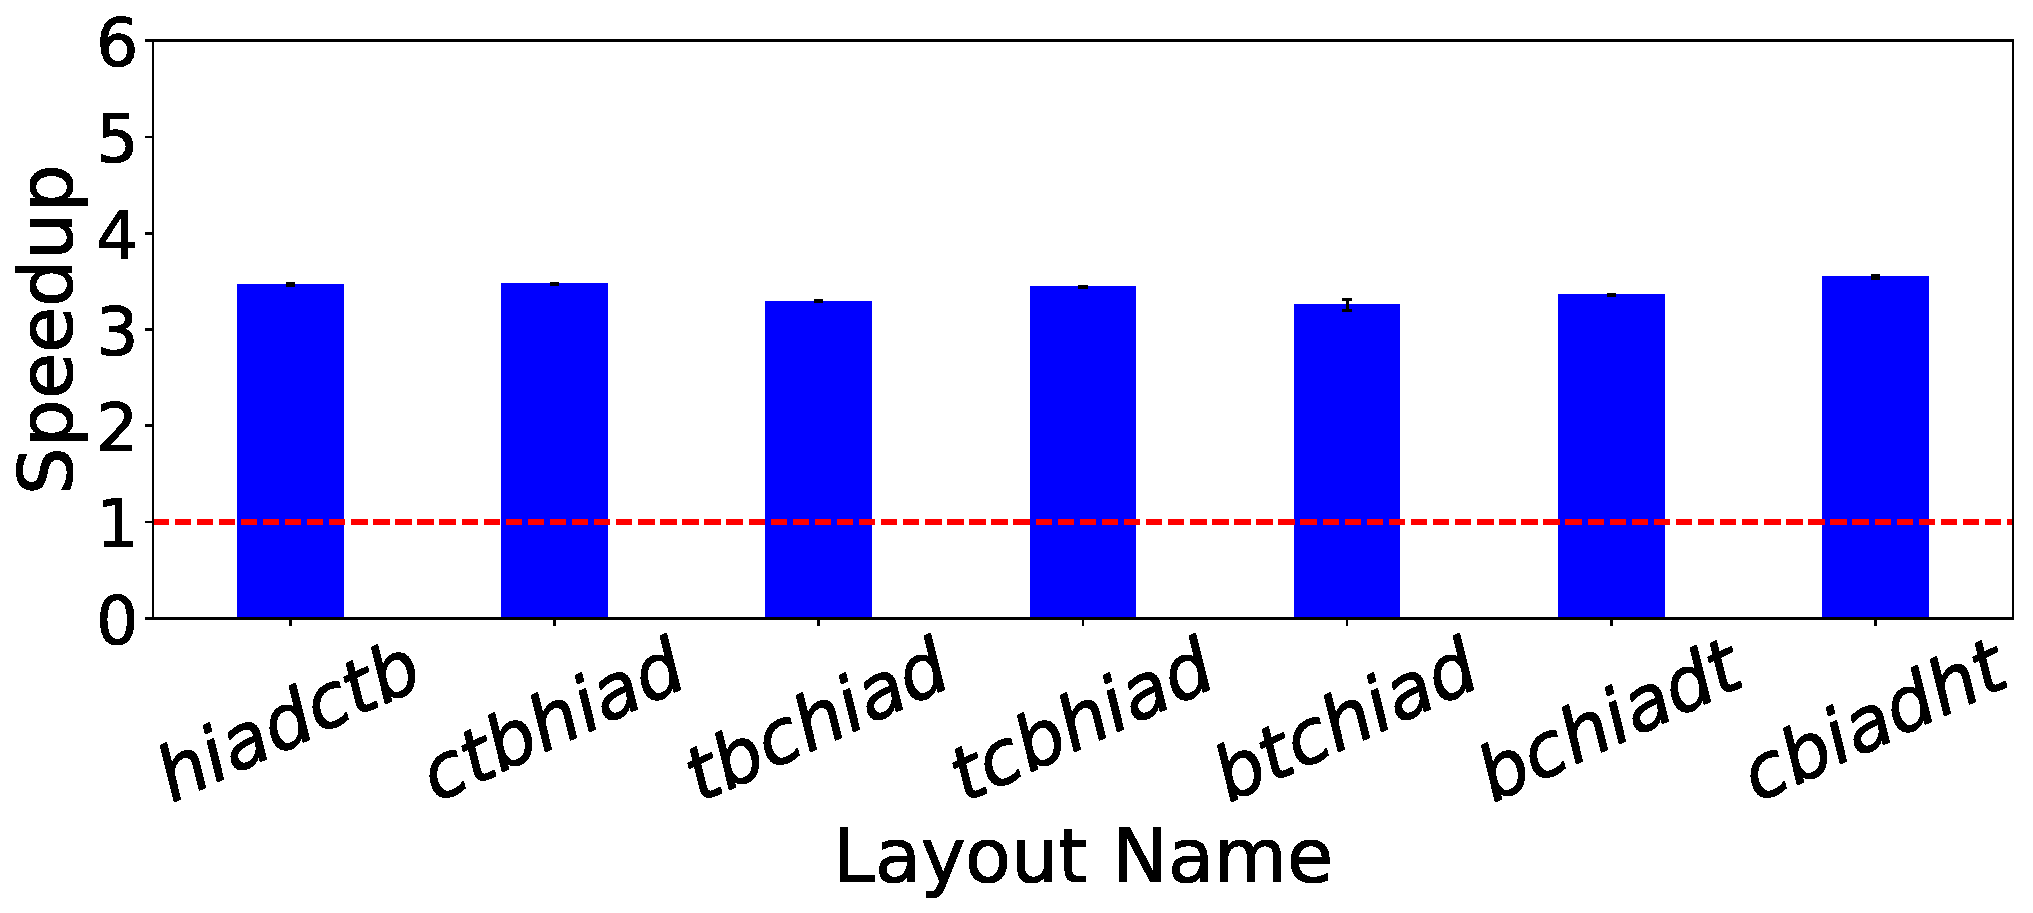
\includegraphics[width=\textwidth]{plots/SpeedupMarmosetGhcFilterBlogs}
		\caption{Filter Blogs Traversal.}
		\label{table:speedupghc-filterblogs}
	\end{subfigure}
	\hfill
	\begin{subfigure}[]{0.3\textwidth}
		\centering
		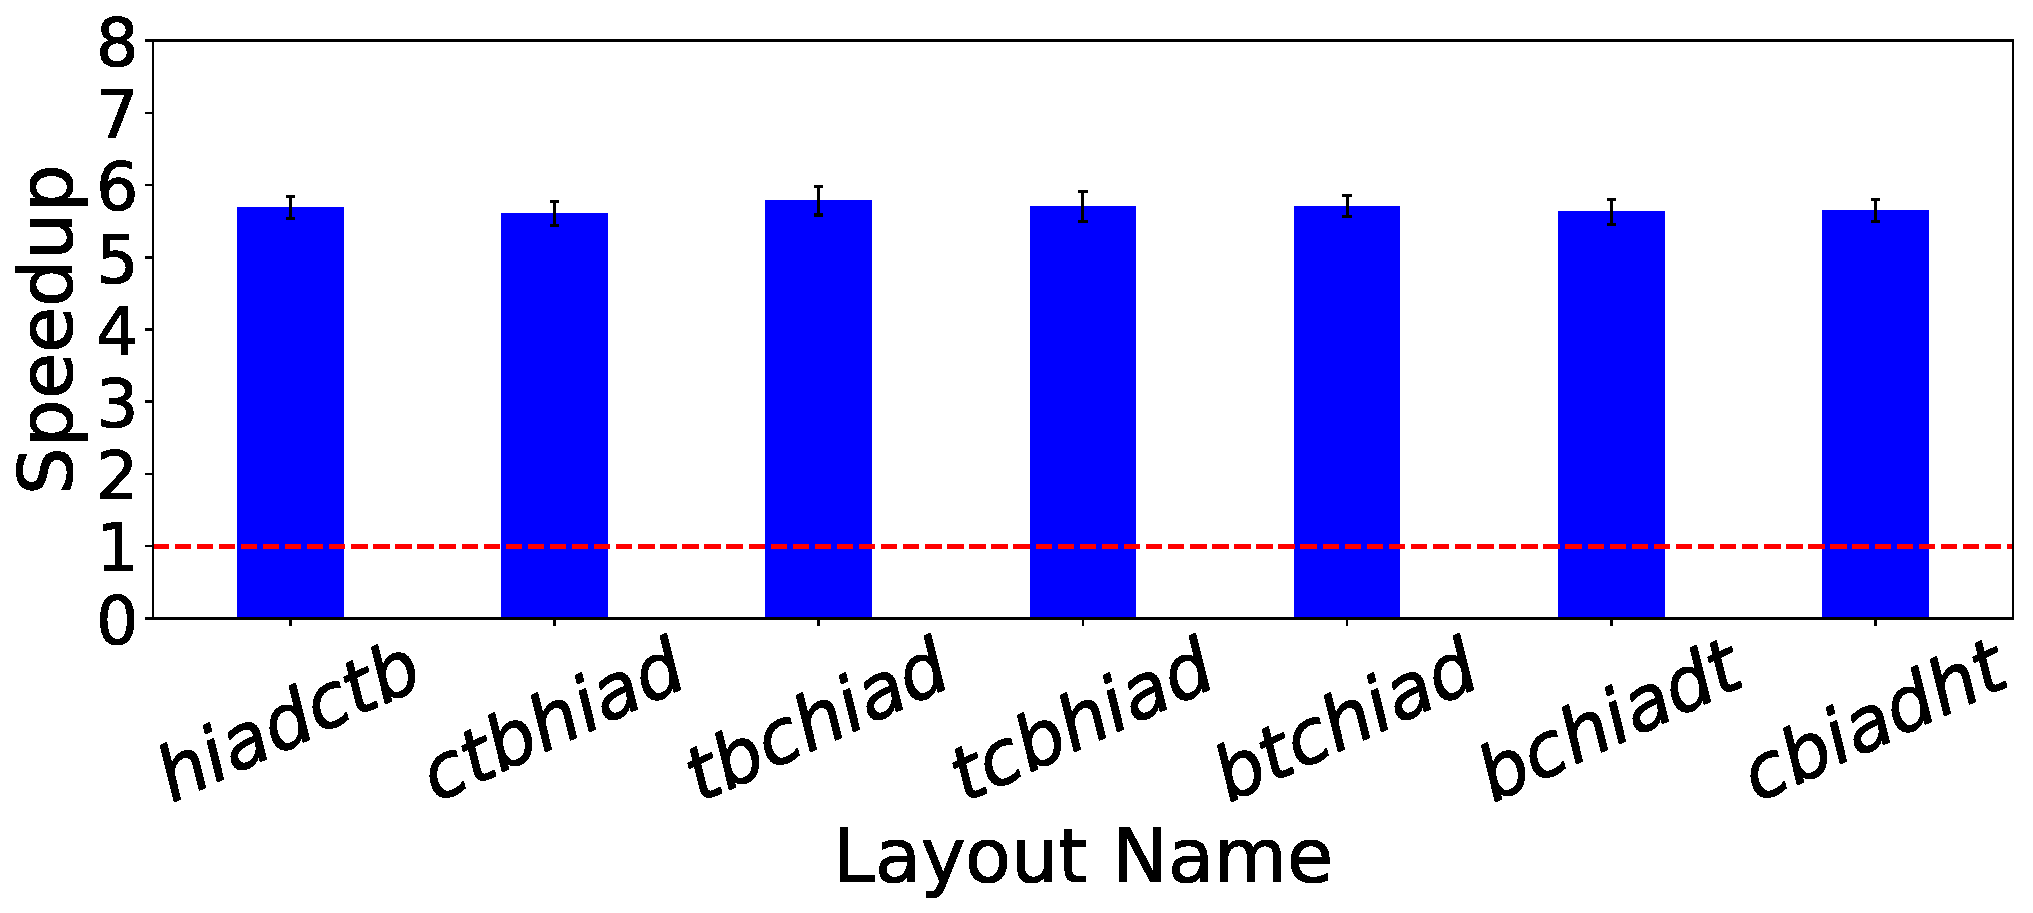
\includegraphics[width=\textwidth]{plots/SpeedupMarmosetGhcContentSearch}
		\caption{Content Search Traversal.}
		\label{table:speedupghc-contentsearch}
	\end{subfigure}
	\hfill
	\begin{subfigure}[]{0.3\textwidth}
		\centering
		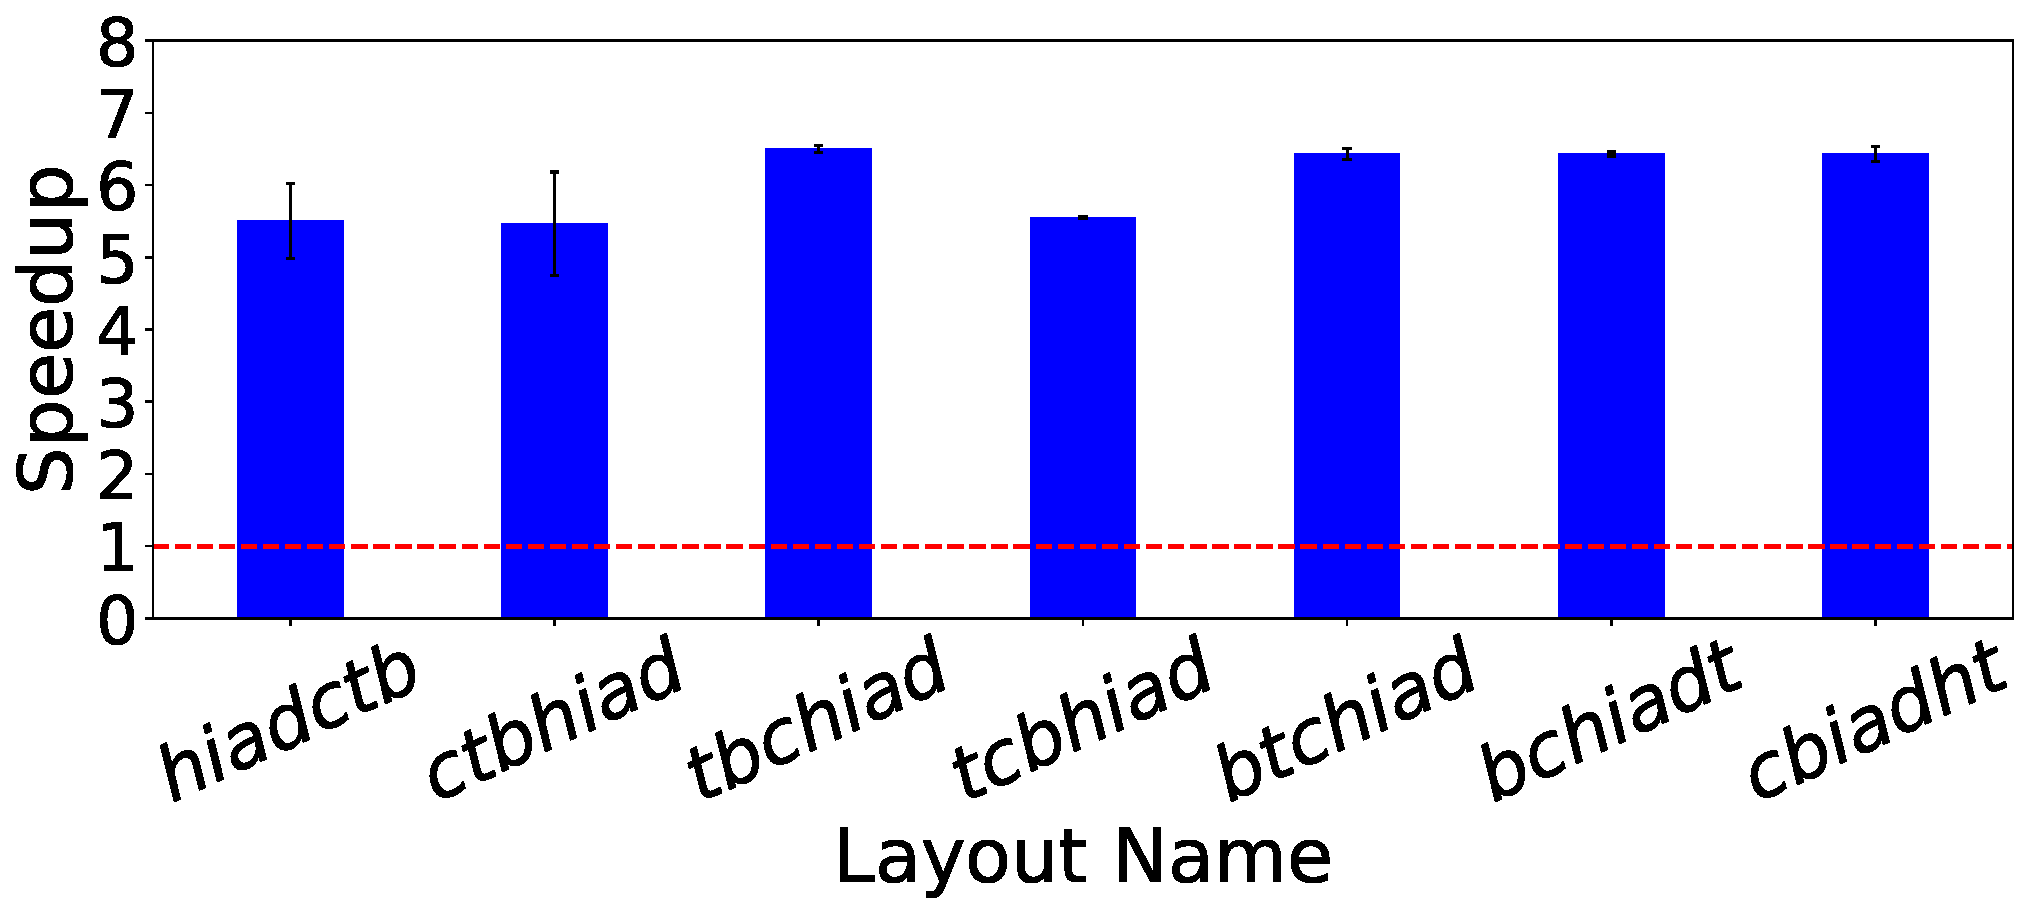
\includegraphics[width=\textwidth]{plots/SpeedupMarmosetGhcTagSearch}
		\caption{Tag Search Traversal.}
		\label{table:speedupghc-tagsearch}
	\end{subfigure}
	   \caption{Performance comparison of \systemSolver with \ghc.}
	   \label{fig:speedupghc}
\end{figure}

\Figref{fig:speedupghc} shows the the speedup of \system over \ghc when evaluated strictly for an apples to apples comparison. We pass the optimization option \textit{-O2} to \ghc while compiling. As shown, the performance of \system is better than \ghc by significant margins for all the layouts and traversals. Since the types in \ghc are \textit{boxed}, such a behavior is expected because it adds more instructions (pointer de-referencing) and results in worse spatial locality.

\subsection{Cache behavior}%
\label{subsec:cache}

% \begin{table}[]
% \setlength{\tabcolsep}{0.0pt} %% default is 6pt
% \centering
% \ra{1}
% \begin{tabular}{@{}p{0.6in}rcrcrcrcrcrcrcrcr@{}}\toprule
% & \multicolumn{1}{c}{\textit{hiadctb}} & 
%  & \multicolumn{1}{c}{\textit{ctbhiad}} &
%  & \multicolumn{1}{c}{\textit{tbchiad}} &
%  & \multicolumn{1}{c}{\textit{tcbhiad}} &
%  & \multicolumn{1}{c}{\textit{btchiad}} &
%  & \multicolumn{1}{c}{\textit{bchiadt}} &
%  & \multicolumn{1}{c}{\textit{cbiadht}} &
%  & \multicolumn{1}{c}{\textit{\systemGreedy}} &
%  & \multicolumn{1}{c}{\small{\systemSolver}}\\ \midrule
% $Filter Blogs$ \\
% $L3\:misses$      &  \textcolor{\myred}{\snum{13688949.333333334}}           &&  \snum{13647736.111111112}  		   &&  {\snum{1670928.0}}   		     &&  {\snum{14134971.666666666}} 									&& \snum{13415231.777777778} 			  && \snum{13646276.888888888} 		 	 &&  \snum{8470132.555555556}      && \textcolor{\myblue}{\snum{1635723.2222222222}} && \snum{1646244.3333333333} \\
% $L3\:accesses$    & \textcolor{\myred}{\snum{17151877.333333332}}            &&  \snum{16509412.777777778}  		   &&  {\snum{7615203.0}}   		     && {\snum{17010157.888888888}} && \snum{15951598.444444444} 			  && \snum{16256262.333333334} 			 &&  \snum{13084325.444444444}               					&& \snum{7555649.111111111}						 && \textcolor{\myblue}{\snum{7549853.444444444}}      	\\
% $L3\:miss\:rate$  & {\fnumthree{0.7981021008545771}} 	&&  \fnumthree{0.8266639337700382}  &&  {\fnumthree{0.21942002071382732}}	 && {\fnumthree{0.8309723965525149}} && \textcolor{\myred}{\fnumthree{0.8409960810197036}}  && \fnumthree{0.8394473839725942}   &&  \fnumthree{0.6473495780519539}     				&& \textcolor{\myblue}{\fnumthree{0.21649009875495365}}		 &&  \fnumthree{0.2180498397018185}    \\
% $Ins$    & {\snum{583470105.5555556}}          				&&  \snum{582533028.4444444}  		   && {\snum{583515820.7777778}}   		 	 && {\snum{581535328.1111112}} 									&& \textcolor{\myblue}{\snum{579646835.3333334}} 		  && \snum{578594445.4444444} 		 	 &&   \textcolor{\myred}{\snum{586877323.4444444}}              		&& \snum{583515815.6666666}									 &&   \snum{583515815.2222222}      \\
% \\
% $Content Search$\\
% $L3\:misses$ 		& {\snum{18901820.666666668}}  								&&  \snum{16680031.111111112}  				&&  {\snum{19447606.444444444}}   					&& {\snum{17056085.111111112}} 					&& \textcolor{\myred}{\snum{21874690.444444444}}    					 		&& {\snum{21780863.777777776}}  			    &&   {\snum{12162521.222222222}}     			&& \textcolor{\myblue}{\snum{11750799.0}}				&& \snum{14249030.333333334}\\
% $L3\:accesses$  	& {\snum{34914340.11111111}}  								&&  \snum{32917716.222222224}  				&&   {{\snum{33649045.222222224}}}  				 	&& {\snum{33867834.88888889}} 					&& \textcolor{\myred}{\snum{36013492.88888889}}     		 					&& {\snum{35869930.44444445}}     		 	&&  {\snum{30606836.666666668}}     			&& \snum{29779038.333333332}				&& \textcolor{\myblue}{\snum{28204429.555555556}} 	\\
% $L3\:miss\:rate$ 	& \fnumthree{0.5413769988638957}        					&&  \fnumthree{0.5067189655110609}  	    &&  {\fnumthree{0.5779541831279367}}         	&& {\fnumthree{0.503607188563056}}       	&& \textcolor{\myred}{\fnumthree{0.6074026341164304}}                     &&  {\fnumthree{0.6072178983316431}}      &&   {\fnumthree{0.39737923113982554}}  		&& \textcolor{\myblue}{\fnumthree{0.39459968009936297}}			&& 	\fnumthree{0.5052054077274056}\\
% $Ins$ 		&  {\snum{5848090746.222222}}				&&  \snum{5837088833.111111}  				&&  {\snum{6776502981.222222}}   					&& {\snum{5844075395.222222}} 					&& \snum{6779241987.666667}   			 				&& \textcolor{\myred}{\snum{6779244909.888889}}            				    &&  \snum{5840089571.111111}     		&& \snum{5840081527.0}					&& \textcolor{\myblue}{\snum{5837021466.666667}}	\\
% \\
% $Tag Search$ \\
% $L3\:misses$ 		& \textcolor{\myred}{\snum{44582803.0}}    							&&  {\snum{43328252.0}}    				&& {\snum{42657869.0}}       && {\snum{39958549.55555555}}   					    && \snum{38454909.55555555} 	    			  			&& {\snum{42618967.666666664}}  		 			&&  \snum{39621576.44444445}  		 	    && \snum{34350961.88888889}			&& \textcolor{\myblue}{\snum{23895872.444444444}}  \\
% $L3\:accesses$ 		& \snum{129939475.33333333}   						 	&&  {\snum{130000024.1111111}}   				&&  \textcolor{\myred}{\snum{212150507.33333334}}      &&  {\snum{134590067.2222222}}   					&& \snum{182445264.2222222} 	      						&& {\snum{148496853.1111111}}   		 			&& {\snum{129647905.44444445}}  			&& \snum{130411896.44444445} 					&& \textcolor{\myblue}{\snum{80664682.55555555}}  \\
% $L3\:miss\:rate$ 	& \textcolor{\myred}{\fnumthree{0.343104379062882}} 					&&  {\fnumthree{0.3332941843377453}}  			&&  \textcolor{\myblue}{\fnumthree{0.20107361295618048}} 			 && {\fnumthree{0.29689077641650796}} 			&& {\fnumthree{0.210775049270211}}  				&& {\fnumthree{0.2870024971827349}}    		&& {\fnumthree{0.30560907489109207}}  && \fnumthree{0.2634035914317251}  	&& \fnumthree{0.29623711006346337}\\
% $Ins$ 		& \snum{22501467492.88889}  							&&  \textcolor{\myblue}{\snum{22497197160.555557}}  	 				&& {\snum{23043358952.11111}}    				 && {{\snum{22497861297.88889}}} 					&& \textcolor{\myred}{\snum{23043512418.0}} 	  						&& {\snum{23041810439.555557}} 	&&  \snum{22498728619.333332} 			 && \snum{22498730120.0}					&& \snum{22487660868.333332}  \\
% \bottomrule
% \end{tabular}
% \caption{Various performance stats (\textit{PAPI}) for different traversals for a subset permutation of different layouts when compiled with \gibbon.
% The last two columns show the cache misses for the layout chosen by \small{\systemGreedy} and \small{\systemSolver} respectively. Legend: h - Header, t - HashTags, b - Blogs, i - TagID, c - Content, a - Author, d - Date. The numbers in \textcolor{\myblue}{Blue} correspond to the min in the row and the numbers in \textcolor{\myred}{Red} correspond to the max in the row.}
% \label{table:filterblogs-papi}
% \end{table}

\begin{table}[t]
	\setlength{\tabcolsep}{3.5pt} %% default is 6pt
	\centering
	\caption{PAPI performance counter statistics (average of 99 runs) for different blog traversals.}
	\begin{tabular}{@{}lrrrrrrrrr@{}}
	\toprule
    \multirow{2}[2]{*}{\thead[l]{Benchmark\\name or metric}}
	  & \multicolumn{7}{c}{{\gibbon}}
      & \multicolumn{2}{c}{{\system}}\\
    \cmidrule(lr){2-8}\cmidrule(lr){9-10}

	 & \multicolumn{1}{c}{\small{{hiadctb}}}
	 & \multicolumn{1}{c}{\small{{ctbhiad}}}
	 & \multicolumn{1}{c}{\small{{tbchiad}}}
	 & \multicolumn{1}{c}{\small{{tcbhiad}}}
	 & \multicolumn{1}{c}{\small{{btchiad}}}
	 & \multicolumn{1}{c}{\small{{bchiadt}}}
	 & \multicolumn{1}{c}{\small{{cbiadht}}}
	 & \multicolumn{1}{c}{\small{{\systemGreedy}}}
	 & \multicolumn{1}{c}{\small{\systemSolver}}\\ 
	\midrule
	\benchname{FilterBlogs} \\
	Ins    & {\snum{583007860.8888888}} &  \snum{582007417.2222222} & {\snum{583006557.5555556}}   & {\snum{581007422.0}} & \textcolor{\myblue}{\snum{579006542.1111112}} & \snum{578007431.3333334} &   \textcolor{\myred}{\snum{586007412.4444444}} & \snum{583006551.4444444} &   \snum{583006570.4444444}    \\
	Cycles    & {\snum{989222808.8888888}} &  \snum{959711380.1111112} & \textcolor{\myblue}{\snum{285081123.8888889}}   & {\snum{1052921958.2222222}} & {\snum{1200439241.3333333}} & \textcolor{\myred}{\snum{1248215771.1111112}} &   {\snum{877792663.1111112}} & \snum{279146331.4444444} &   \snum{289017037.7777778}    \\
	L2\:DCM    & {\snum{11185155.333333334}} &  \snum{11510078.222222222} & {\snum{938489.3333333334}}   & \textcolor{\myred}{\snum{13337049.333333334}} & {\snum{12928602.222222222}} & \snum{13065840.0} &   {\snum{7789525.777777778}} & \snum{889989.7777777778} &   \textcolor{\myblue}{\snum{874607.7777777778}}    \\
	\\
	\benchname{EmphContent}\\
	Ins    & {\snum{5845022229.888889}} &  \snum{5834021360.444445} & {\snum{6776362325.666667}}   & {\snum{5841021767.888889}} & {\snum{6779241706.444445}} & \textcolor{\myred}{\snum{6779244615.888889}} &   \textcolor{\myblue}{\snum{5837021292.777778}} & \snum{5837021295.333333} &   \snum{5837021366.222222}    \\
	Cycles   & {\snum{2892647565.888889}} &  \snum{2738456405.4444447} & {\snum{4272337912.0}}   & {\snum{2842427055.6666665}} & \textcolor{\myred}{\snum{4340585270.333333}} & \snum{4291414051.5555553} &   \textcolor{\myblue}{\snum{2056621185.3333333}} & \snum{2061807292.6666667} &   \snum{2812417391.5555553}    \\
	L2\:DCM    & {\snum{12800140.0}} &  \snum{10780195.333333334} & {\snum{20295265.222222224}}   & {\snum{13283107.333333334}} & \textcolor{\myred}{\snum{20549853.111111112}} & \snum{20994551.666666668} &   \textcolor{\myblue}{\snum{7727582.888888889}} & \snum{7663269.0} &   \snum{10702561.555555556}    \\
	\\
	\benchname{TagSearch} \\
	Ins    & {\snum{22490860539.77778}} &  \textcolor{\myblue}{\snum{22487260185.555557}} & \textcolor{\myred}{\snum{23043358250.333332}}   & {\snum{22487260291.333332}} & {\snum{23043009879.0}} & \snum{23041811630.22222} &   {\snum{22488060134.77778}} & \snum{22487659963.444443} &   \snum{22487659965.0}    \\
	Cycles    & {\snum{8587261902.555555}} &  \snum{8593729939.88889} & {\snum{9609104561.222221}}   & \textcolor{\myblue}{\snum{7288093434.666667}} & {\snum{9607367711.666666}} & \textcolor{\myred}{\snum{9748577539.11111}} &   {\snum{7883183997.666667}} & \snum{7609921682.888889} &   \snum{7568236436.222222}    \\
	L2\:DCM    & {\snum{20227011.777777776}} &  \snum{20621886.333333332} &  \textcolor{\myred}{\snum{39956792.44444445}}   & \textcolor{\myblue}{\snum{10612695.222222222}} & {\snum{28602975.777777776}} & \snum{26479819.222222224} &  {\snum{16392591.777777778}} & \snum{12885043.444444444} &   \snum{12753814.333333334}    \\
	\bottomrule
	\end{tabular}
	\label{table:filterblogs-papi}
	\end{table}

The results from earlier sections demonstrate that \system's layout choices improve run-time performance. This section investigates {\em why} performance improves. The basic premise of \system's approach to layout optimization is to concentrate on minimizing how often a traversal needs to backtrack or skip ahead while processing a buffer. By minimizing this jumping around, we expect to see improvements from two possible sources. First, we expect to see an improvement in instruction counts, as an optimized layout should do less pointer chasing. Second, we expect to see an improvement in L2 and L3 cache utilization: both fewer misses (due to improved spatial locality and prefetching) and fewer accesses (due to improved locality in higher level caches).

Table~\ref{table:filterblogs-papi} shows that our main hypothesis is borne out and the optimal layout has fewer
%To substantiate this hypothesis we collect performance counters for various layouts
%L3 accesses and L3 misses:
L2 data cache misses%
\footnote{Since PAPI, the processor counters framework, does not completely support latest AMD processors yet, we were unable to obtain L3 cache misses, only the L2 DCM counter was available.}:
a better layout promotes better locality. Interestingly, we do not observe a similar effect for instruction count. While different layouts differ in instruction counts, the difference is slight. We suspect this light effect of a better layout may be due to \gibbon's current implementation, which often dereferences pointers even if a direct access in the buffer would suffice.

\subsection{Tradeoffs between \system's solver and greedy optimization}%
\label{subsec:heuristic-tradeoffs}

To understand the difference between the layout chosen by \systemSolver and \systemGreedy we now take a closer look at the tag search traversal shown in Table~\ref{table:blog-traversals}.
Here, both versions choose two different layouts with different performance implications. \systemSolver chooses the layout \textbf{\textit{tbchiad}} whereas \systemGreedy chooses 
the layout \textbf{\textit{tcbhiad}}. The mechanics of why can be explained using our running example (Figure~\ref{fig:blog-traversal}) which is essentially a simplified version of the 
traversal shown in the evaluation. Figure~\ref{graph:running-access} shows the access graph for this traversal. \systemSolver generates constraints 
outlined in Section~\ref{design:genconstraints} that lead to the layout \textbf{\textit{tbchiad}}. On the other hand, \systemGreedy starts at the root node of the graph and greedily chooses the next child to traverse. 
The order in which nodes of the graph are visited fixes the order of fields in the data constructor. In this case, the root node is \lstinline|HashTags| which makes it the first field in the greedy 
layout, next, the greedy heuristic picks the \lstinline|Content| field making it the second field and finally followed by the \lstinline|BlogList| field.

In \figref{table:compiletimes} (p.~\pageref{table:compiletimes}), we show the compile times for different layout and traversal combinations when compiled with \gibbon, \systemGreedy and \systemSolver respectively as
a measure of relative costs. The compile times for \systemSolver include the time to generate the control flow graph, the field access graph, the solver time and the time to re-order the datatype in the code.
The solver times are in the order of the number of fields in a data constructor and not the program size. Hence, the solver adds relatively low overhead.
Since the compiler does an IO call to the python solver, there is room for improvement in the future to lower these times. 
For instance, we could directly perform \textit{FFI} calls to the CPLEX solver by lowering the constraints to C code. 
This would be faster and safer than the current implementation. In addition, during the global optimization, we call the solver on each data constructor as of the moment, 
we could further optimize this by sending constraints for all data constructors at once and doing just one solver call. 

Although the cost of \system's solver based optimization is higher than the greedy approach, it is a complementary approach 
which may help the user find a better layout at the cost of compile time. On the other hand, if the user wishes to optimize 
for the compile time, they should use the greedy heuristic.


\subsection{Discussion: Scale of Evaluation}%
\label{subsec:scale-eval}

\system's approach for finding the best layout for densely presented
data is language agnostic, but the evaluation has to be language specific.
Hence, we implemented the approach inside a most-developed (to our
knowledge) compiler supporting dense representations of recursive datatypes, the
Gibbon compiler. Our evaluation is heavily influenced by this.

At the time of writing, the scale of evaluation is limited by a number of
Gibbon-related restrictions.
Gibbon is meant as a tree traversal accelerator~\cite{gibbon} and
its original suite of benchmarks served as a basis and inspiration for
evaluation of \system.
``Big'' end-to-end projects (e.g. compilers, web servers, etc.)
have not been implemented in Gibbon and, therefore, are out of reach for us.
If someone attempted to implement such a project using Gibbon,
they would have to extend the compiler to support many realistic features:
modules, FFI, general I/O, networking.
Alternatively, one could integrate Gibbon into an existing realistic compiler
as an optimization pass or a plugin.
For instance, the Gibbon repository has some preliminary work for integrating as a
GHC plugin\footnote{%
  \url{https://github.com/iu-parfunc/gibbon/tree/24c41c012a9c33bff160e54865e83a5d0d7867dd/gibbon-ghc-integration}
}, but it is far from completion.
In any case, the corresponding effort is simply too big.
%
%Overall, we do not see a feasible way to offer a larger-scale evaluation.
Overall, the current \system evaluation shows that our approach is viable.
